\section{Техническое задание}

\subsection{Основание для разработки}

Основанием для разработки является задание на выпускную квалификационную работу бакалавра <<Разработка веб-платформы для автоматизации бизнес-процессов управления персоналом компании>>. Проект реализуется в рамках производственной практики студента в компании ООО <<ВТИ-Сервис>>.

\subsection{Цель и назначение разработки}

Целью проекта является разработка и внедрение веб-платформы, которая обеспечит эффективное управление внутренними коммуникациями и координацией персонала.

Задачи разработки включают:

\begin{enumerate}
  \item Создание единого доступа ко всем внутренним бизнес-сервисам.
  \item Централизация данных и снижение фрагментированности инструментов.
  \item Повышение прозрачности процессов и контроль выполнения задач.
  \item Ускорение документооборота и взаимодействия между сотрудниками.
  \item Внедрение интуитивного интерфейса и адаптивной архитектуры.
\end{enumerate}

\subsection{Функциональные задачи}

Разрабатываемая веб-платформа должна включать разные сервисные модули, позволяющие эффективно работать сотруднику в компании, коммуницировать с другими сотрудниками, заводить и следить за задачами.

\subsubsection{Почта}

Назначение: модуль для внутренней и внешней переписки сотрудников.

Функциональность:
\begin{itemize}
  \item просмотр входящих, отправленных, черновиков и пользовательских папок;
  \item отправка писем одному или нескольким адресатам;
  \item прикрепление файлов с устройства или из сервиса <<Файлы>>;
  \item сохранение черновиков и их редактирование;
  \item фильтрация писем по дате, отправителю, теме;
  \item возможность перемещения писем между папками;
  \item интеграция с контактами (автозаполнение).
\end{itemize}

Варианты использования:
\begin{enumerate}
  \item Сотрудник пишет письмо руководителю, прикладывает отчёт, отправляет.
  \item Пользователь ищет письмо по теме и сохраняет его в отдельную папку.
  \item При получении письма с вложением — загружает файл во внутреннее хранилище.
\end{enumerate}

Бизнес-правила:
\begin{enumerate}
  \item Максимальный размер вложения — 10 МБ.
  \item Письма с внешними доменами логируются отдельно.
  \item При отсутствии темы система предлагает указать её перед отправкой.
  \item Подпись подставляется автоматически на основе профиля пользователя.
\end{enumerate}

Ограничения:
\begin{enumerate}
  \item Запрет на пересылку писем вне домена без разрешения администратора.
  \item Вложения проверяются встроенным антивирусом.
  \item Недоступность функций без активного интернет-соединения.
\end{enumerate}

\subsubsection{Контакты}

Назначение: централизованная адресная книга сотрудников компании.

Функциональность:
\begin{itemize}
  \item добавление, редактирование и удаление контактов;
  \item поиск и фильтрация по имени, отделу, должности;
  \item просмотр статуса (в сети/нет), контактной информации;
  \item быстрый запуск общения: письмо, задача, вызов.
\end{itemize}

Варианты использования:
\begin{enumerate}
  \item Руководитель ищет сотрудника по должности и ставит ему задачу.
  \item Пользователь сохраняет нового партнёра в адресную книгу.
  \item Секретарь создаёт общую папку контактов отдела.
\end{enumerate}

Бизнес-правила:
\begin{enumerate}
  \item Только пользователи с ролью "Администратор" могут создавать общие контакты.
  \item Каждый контакт должен иметь уникальный email.
  \item Контакт может быть связан с задачами, письмами и ВКС.
\end{enumerate}

Ограничения:
\begin{enumerate}
  \item Запрет на удаление контактов, связанных с активными задачами.
  \item Ограничение количества создаваемых папок — не более 50.
  \item Только латинские и кириллические символы в имени.
\end{enumerate}

\subsubsection{Проекты}

Назначение: модуль управления задачами и проектной деятельностью.

Функциональность:
\begin{itemize}
  \item создание и редактирование проектов;
  \item создание задач с указанием исполнителя, приоритета, сроков;
  \item иерархия задач и подзадач;
  \item фильтрация задач по статусу, приоритету, исполнителю;
  \item отслеживание выполнения и комментирование задач.
\end{itemize}

Варианты использования:
\begin{enumerate}
  \item Менеджер создаёт проект и назначает исполнителей.
  \item Сотрудник обновляет статус своей задачи.
  \item Участник оставляет комментарий с прикреплением файла.
\end{enumerate}

Бизнес-правила:
\begin{enumerate}
  \item Каждая задача должна принадлежать проекту.
  \item Только автор задачи может её удалить.
  \item Задачи можно закрывать только при заполнении обязательных полей.
\end{enumerate}

Ограничения:
\begin{enumerate}
  \item Ограничение по числу задач в одном проекте — 500.
  \item Отсутствие связи с календарём — запрещено создавать задачу.
  \item Отсутствие права — блокирует возможность назначения исполнителя.
\end{enumerate}

\subsubsection{Календарь}

Назначение: организация мероприятий, событий и встреч.

Функциональность:
\begin{itemize}
  \item создание, редактирование, удаление событий;
  \item указание участников, времени, места, описания;
  \item напоминания, повторяющиеся события;
  \item интеграция с задачами и видеоконференциями.
\end{itemize}

Варианты использования:
\begin{enumerate}
  \item Сотрудник планирует встречу с отделом на пятницу.
  \item Ассистент создаёт событие и прикрепляет к нему задачу.
  \item Пользователь подключается к ВКС через событие.
\end{enumerate}

Бизнес-правила:
\begin{enumerate}
  \item Событие без даты и времени не может быть сохранено.
  \item Только организатор может изменить участников.
  \item Событие, начавшееся более 24 часов назад, не редактируется.
\end{enumerate}

Ограничения:
\begin{enumerate}
  \item Максимум 100 участников на событие.
  \item Поддерживаются только даты в пределах текущего года.
  \item Нельзя создавать события без заголовка.
\end{enumerate}

\subsubsection{Файлы}

Назначение: централизованное хранение файлов и документов.

Функциональность:
\begin{itemize}
  \item загрузка, скачивание, удаление файлов;
  \item создание папок и организация структуры хранения;
  \item настройка прав доступа (просмотр, редактирование);
  \item отображение истории изменений и авторов.
\end{itemize}

Варианты использования:
\begin{enumerate}
  \item Сотрудник загружает отчёт и делится им с руководителем.
  \item Пользователь сохраняет прикрепление из письма в папку.
  \item Команда работает над одним документом с доступом на редактирование.
\end{enumerate}

Бизнес-правила:
\begin{enumerate}
  \item Размер одного файла не более 100 МБ.
  \item Удалённые файлы хранятся в корзине 30 дней.
  \item Расширения .exe, .bat — запрещены.
\end{enumerate}

Ограничения:
\begin{enumerate}
  \item Максимум 10 ГБ хранилища на одного пользователя.
  \item Ограничение по структуре вложенности — не более 5 уровней.
  \item Нет возможности редактировать файлы онлайн.
\end{enumerate}

\subsubsection{Разговоры}

Назначение: обмен сообщениями в рамках рабочих групп и диалогов.

Функциональность:
\begin{itemize}
  \item создание чатов, каналов, групповых обсуждений;
  \item отправка и получение сообщений, файлов, ссылок;
  \item уведомления, индикация непрочитанных сообщений;
  \item поддержка эмодзи, markdown, реакций.
\end{itemize}

Варианты использования:
\begin{enumerate}
  \item Отдел создаёт рабочий чат для обсуждения проекта.
  \item Сотрудник пишет личное сообщение коллеге.
  \item Канал используется для корпоративных объявлений.
\end{enumerate}

Бизнес-правила:
\begin{enumerate}
  \item Только модераторы могут удалять сообщения других пользователей.
  \item Каналы могут быть публичными или приватными.
  \item История сообщений хранится бессрочно.
\end{enumerate}

Ограничения:
\begin{enumerate}
  \item Размер одного сообщения — до 10 000 символов.
  \item Число участников в группе — до 500.
  \item Без авторизации доступ к чатам невозможен.
\end{enumerate}

\subsubsection{Видеоконференцсвязь (ВКС)}

Назначение: проведение видеовстреч с возможностью демонстрации экрана.

Функциональность:
\begin{itemize}
  \item создание и вход в конференцию;
  \item приглашение участников из контактов;
  \item демонстрация экрана, чат во время встречи;
  \item запись встречи (если разрешено).
\end{itemize}

Варианты использования:
\begin{enumerate}
  \item Организатор создаёт встречу и отправляет ссылку коллегам.
  \item Участники обсуждают проект в ВКС с возможностью совместного просмотра.
  \item Использование ВКС для удалённого собеседования.
\end{enumerate}

Бизнес-правила:
\begin{enumerate}
  \item Организатор — единственный, кто может завершить встречу для всех.
  \item Максимальная длительность конференции — 4 часа.
  \item Запись сохраняется только по согласию всех участников.
\end{enumerate}

Ограничения:
\begin{enumerate}
  \item До 50 участников одновременно.
  \item Требуется доступ к микрофону и камере.
  \item Только сотрудники компании могут создавать встречи.
\end{enumerate}

\subsubsection{Настройки}

Назначение: управление профилем, конфиденциальностью и интерфейсом.

Функциональность:
\begin{itemize}
  \item редактирование имени, почты, пароля;
  \item смена темы (светлая/тёмная), цветовой палитры;
  \item установка предпочтительного языка;
  \item настройки конфиденциальности, уведомлений.
\end{itemize}

Варианты использования:
\begin{enumerate}
  \item Сотрудник включает тёмную тему и отключает звуковые уведомления.
  \item Пользователь меняет email для входа.
  \item Владелец аккаунта устанавливает личную подпись для писем.
\end{enumerate}

Бизнес-правила:
\begin{enumerate}
  \item Изменения вступают в силу только после подтверждения.
  \item Тема и язык сохраняются в настройках пользователя.
  \item Администраторы могут блокировать часть параметров.
\end{enumerate}

Ограничения:
\begin{enumerate}
  \item Нельзя установить недопустимый язык (поддерживаются только ru/en).
  \item Изменение почты требует повторной авторизации.
  \item Ограничение на длину подписи — 1000 символов.
\end{enumerate}

\subsubsection{Панель управления}

Назначение: стартовая страница с доступом к ключевой информации и виджетам.

Функциональность:
\begin{itemize}
  \item отображение виджетов из всех сервисов;
  \item персонализация: выбор нужных модулей;
  \item быстрый доступ к письмам, задачам, событиям;
  \item отображение уведомлений.
\end{itemize}

Варианты использования:
\begin{enumerate}
  \item Руководитель отслеживает задачи и письма на одной странице.
  \item Сотрудник скрывает ненужные виджеты и закрепляет избранные.
  \item Уведомления на панели помогают не пропустить важное.
\end{enumerate}

Бизнес-правила:
\begin{enumerate}
  \item Настройки панели сохраняются в профиле.
  \item Виджеты обновляются в реальном времени.
  \item Доступ к данным зависит от прав пользователя.
\end{enumerate}

Ограничения:
\begin{enumerate}
  \item Одновременно можно отобразить не более 10 виджетов.
  \item Без авторизации панель не доступна.
  \item Обновление панели происходит каждые 10 секунд.
\end{enumerate}


\subsection{Требования пользователя к интерфейсу веб-платформы}

Интерфейс должен обеспечивать:
\begin{itemize}
  \item интуитивную навигацию между модулями;
  \item адаптивную вёрстку для десктопов и мобильных устройств;
  \item визуальное разграничение ролей пользователей;
  \item поддержку светлой и тёмной темы.
\end{itemize}

Макет интерфейса сервиса <<Почта>> представлена на рисунке \ref{templ:image1} и состоит из:
\begin{itemize}
  \item кнопки для отправки письма(1);
  \item списка папок (2);
  \item окна для просмотра писем из выбранной папки (3);
  \item компонента пагинации (4);
  \item компонента навигации по сервисам (5).
\end{itemize}
\begin{figure}[H]
	\centering
	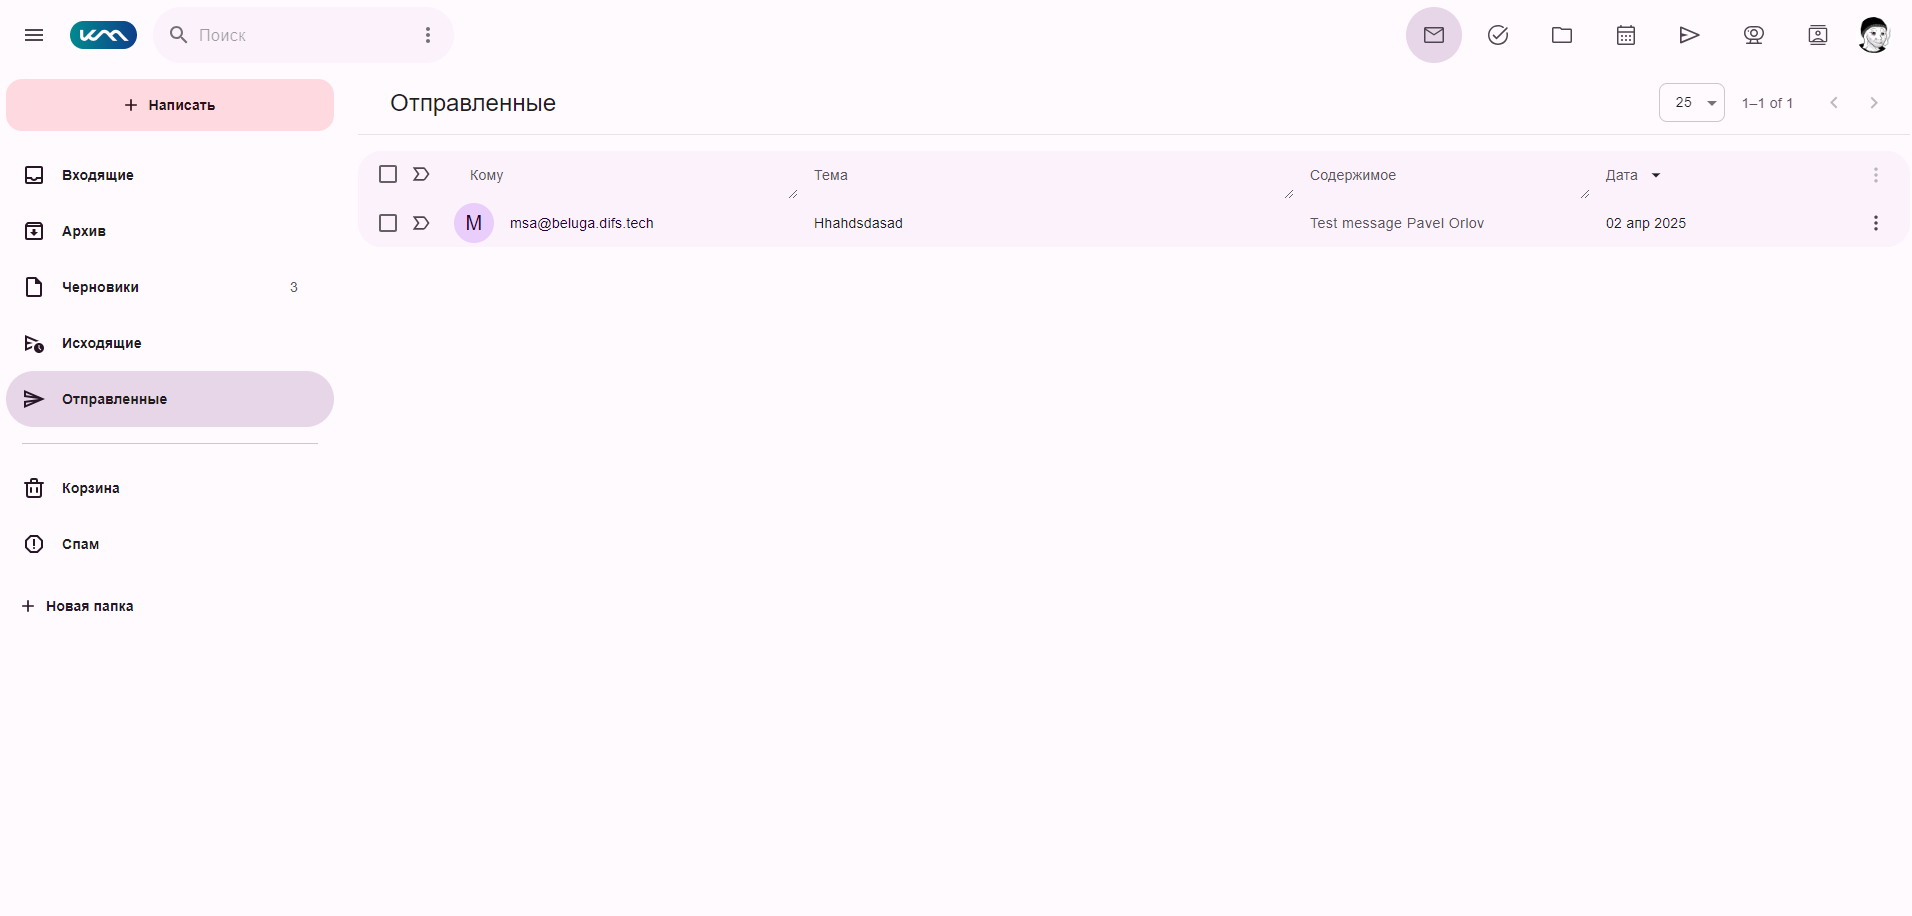
\includegraphics[width=1\linewidth]{images/почта}
	\caption{Макет интерфейса сервиса <<Почта>>}
	\label{templ:image1}
\end{figure}

Макет интерфейса написания письма в сервисе <<Почта>> представлена на рисунке \ref{templ:image1b} и состоит из:
\begin{itemize}
  \item окна ввода письма (1);
  \item поля ввода адресата (2);
  \item кнопок для ввода адресата с целью получения копии/скрытой копии (3);
  \item поля для ввода темы письма (4);
  \item окна для ввода тела письма (5);
  \item кнопок для отправки/сохранения письма в черновик (6);
  \item кнопок для прикрепления файла с компьютера или из сервиса <<Файлы>> (7);
  \item кнопки для закрытия окна без сохранения письма в черновик (8).
\end{itemize}
\begin{figure}[H]
	\centering
	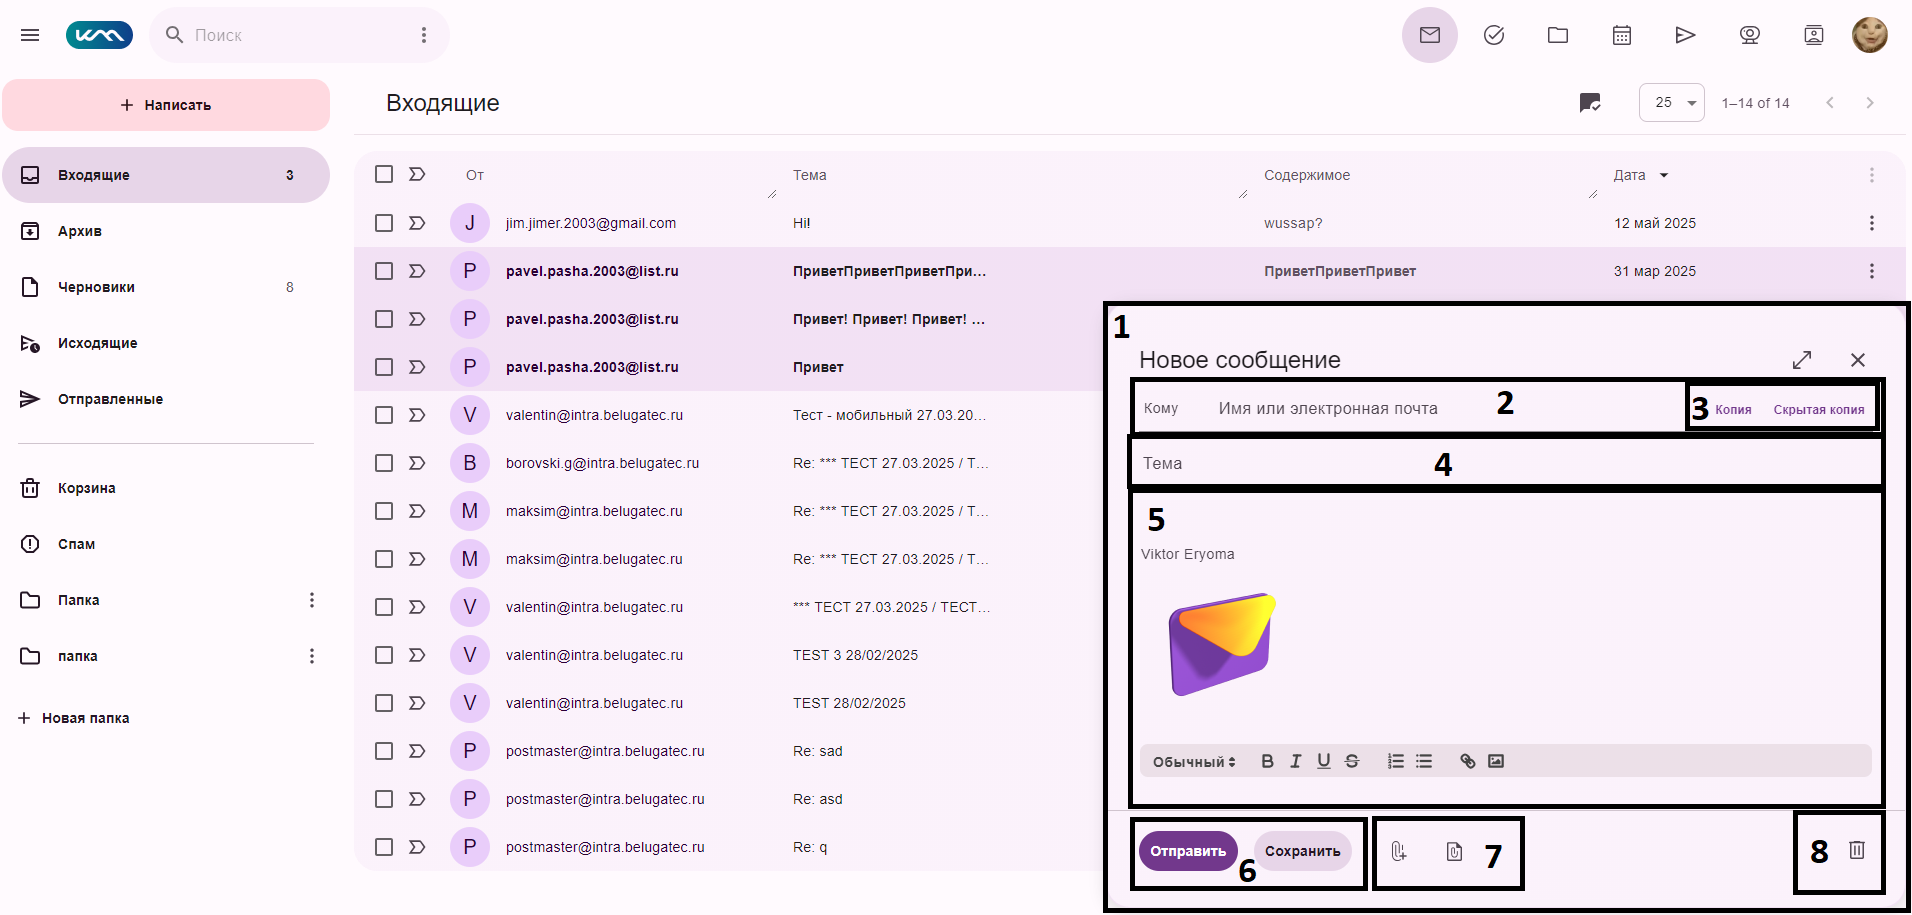
\includegraphics[width=1\linewidth]{images/почта2}
	\caption{Макет интерфейса написания письма}
	\label{templ:image1b}
\end{figure}

Макет интерфейса прикрепление файла из сервиса <<Файлы>> в сервисе <<Почта>> представлена на рисунке \ref{templ:image1c} и состоит из:
\begin{itemize}
  \item всплывающего окна(1);
  \item разделов с файлами (2);
  \item компонента файла с функцией выбора (3);
  \item кнопок для прикрепления файла (4).
\end{itemize}
\begin{figure}[H]
	\centering
	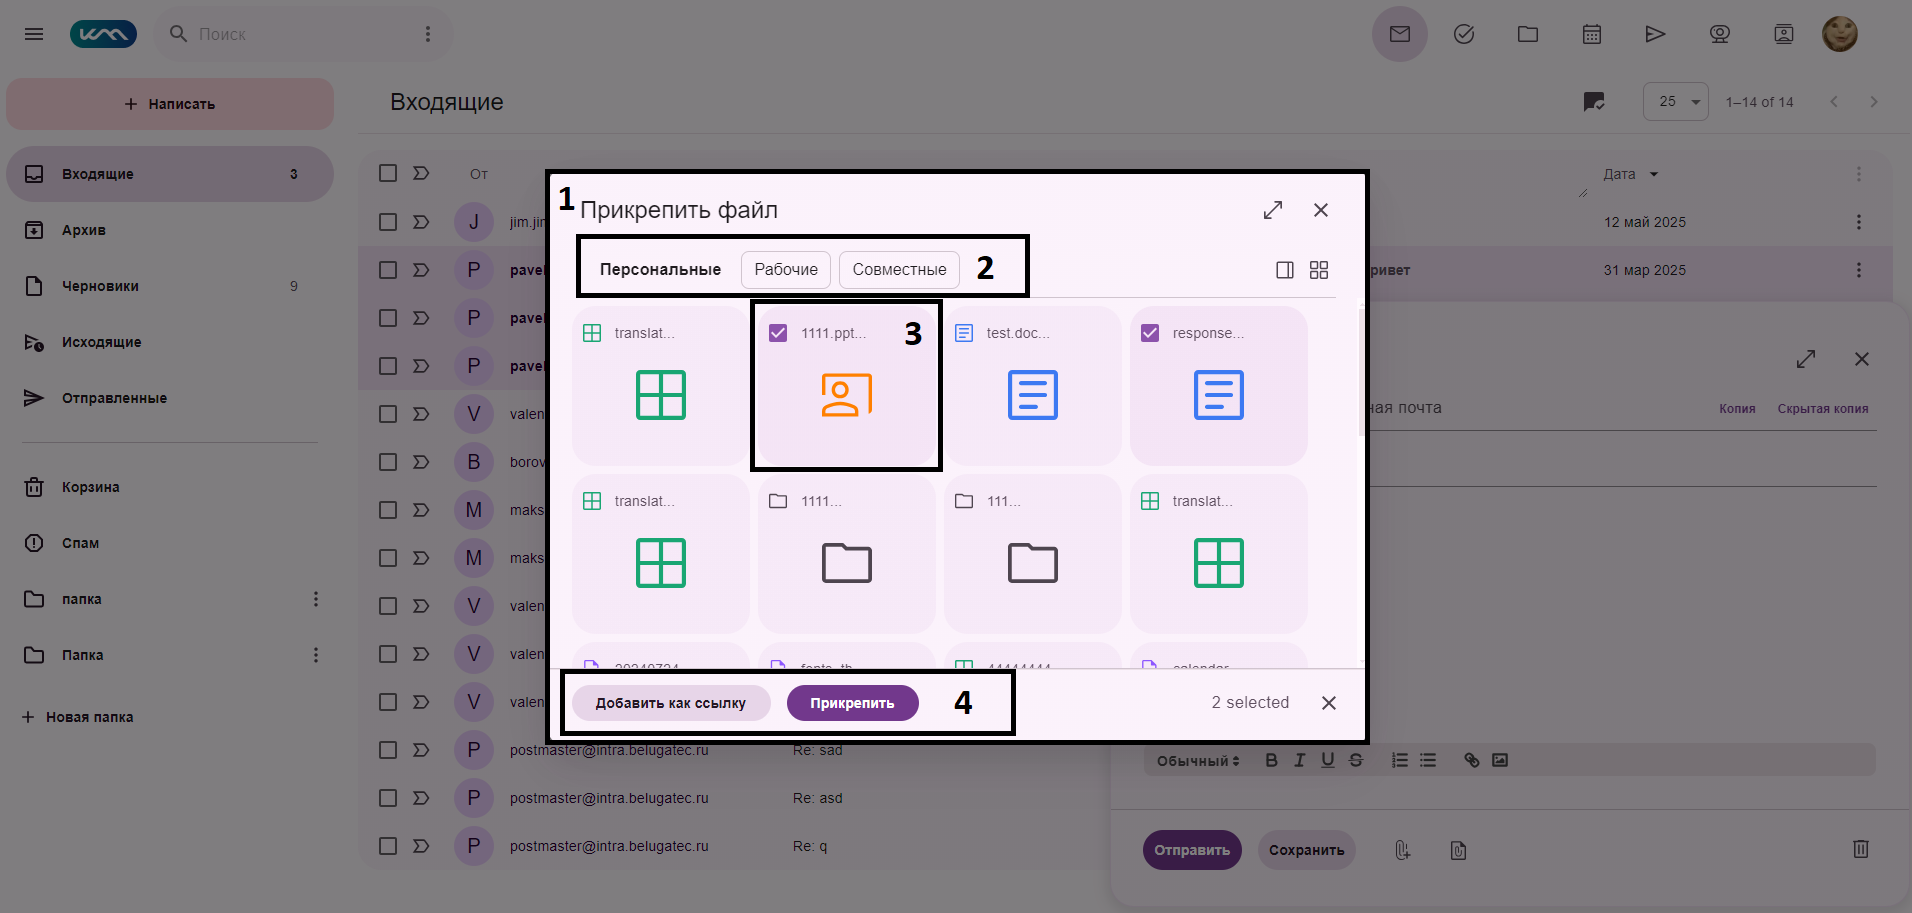
\includegraphics[width=1\linewidth]{images/почта3}
	\caption{Макет интерфейса прикрепление файла}
	\label{templ:image1c}
\end{figure}

Макет интерфейса создания папки в сервисе <<Почта>> представлена на рисунке \ref{templ:image1d} и состоит из:
\begin{itemize}
  \item всплывающего окна(1);
  \item поля ввода названия папки (2);
  \item кнопок действий (3).
\end{itemize}
\begin{figure}[H]
	\centering
	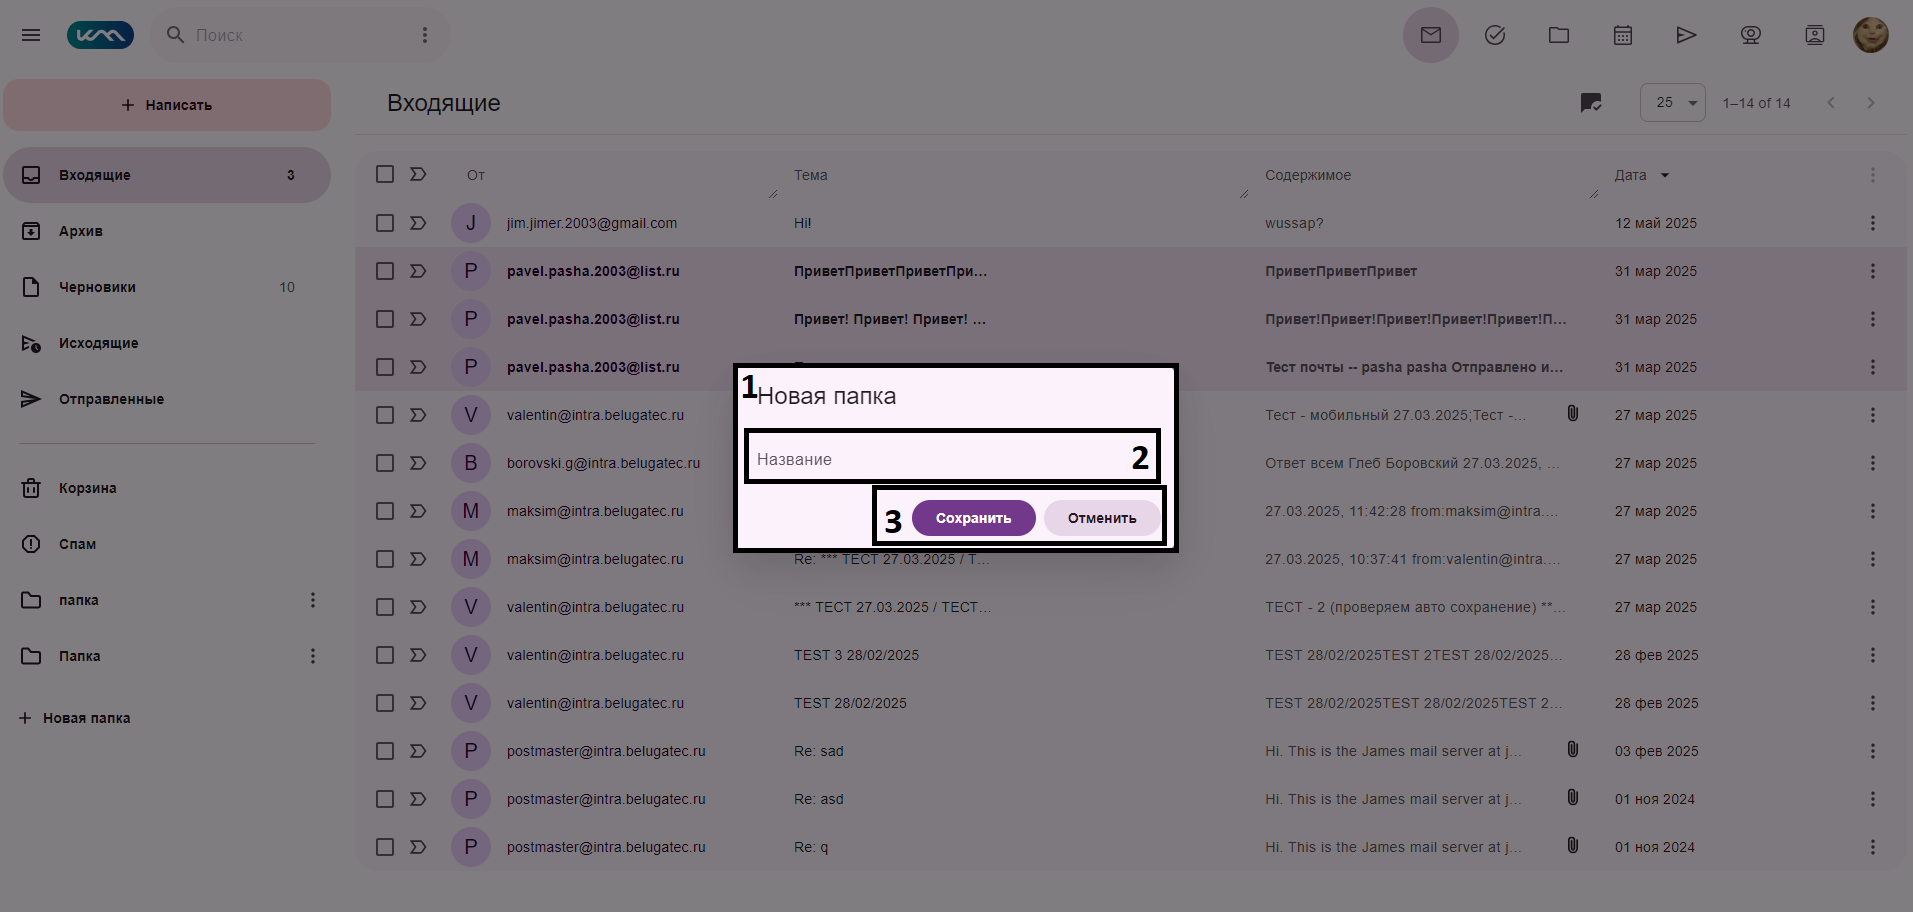
\includegraphics[width=1\linewidth]{images/почта4}
	\caption{Макет интерфейса создания папки}
	\label{templ:image1d}
\end{figure}

Макет интерфейса сервиса <<Видеоконференцсвязь>> представлена на рисунке \ref{templ:image2} и состоит из:
\begin{itemize}
  \item компонента навигации по сервисам (1);
  \item поля для ввода названия комнаты (2);
  \item кнопки для подключения к комнате (3);
  \item кнопки для подключения к запланированным встречам (4).
\end{itemize}
\begin{figure}[H]
	\centering
	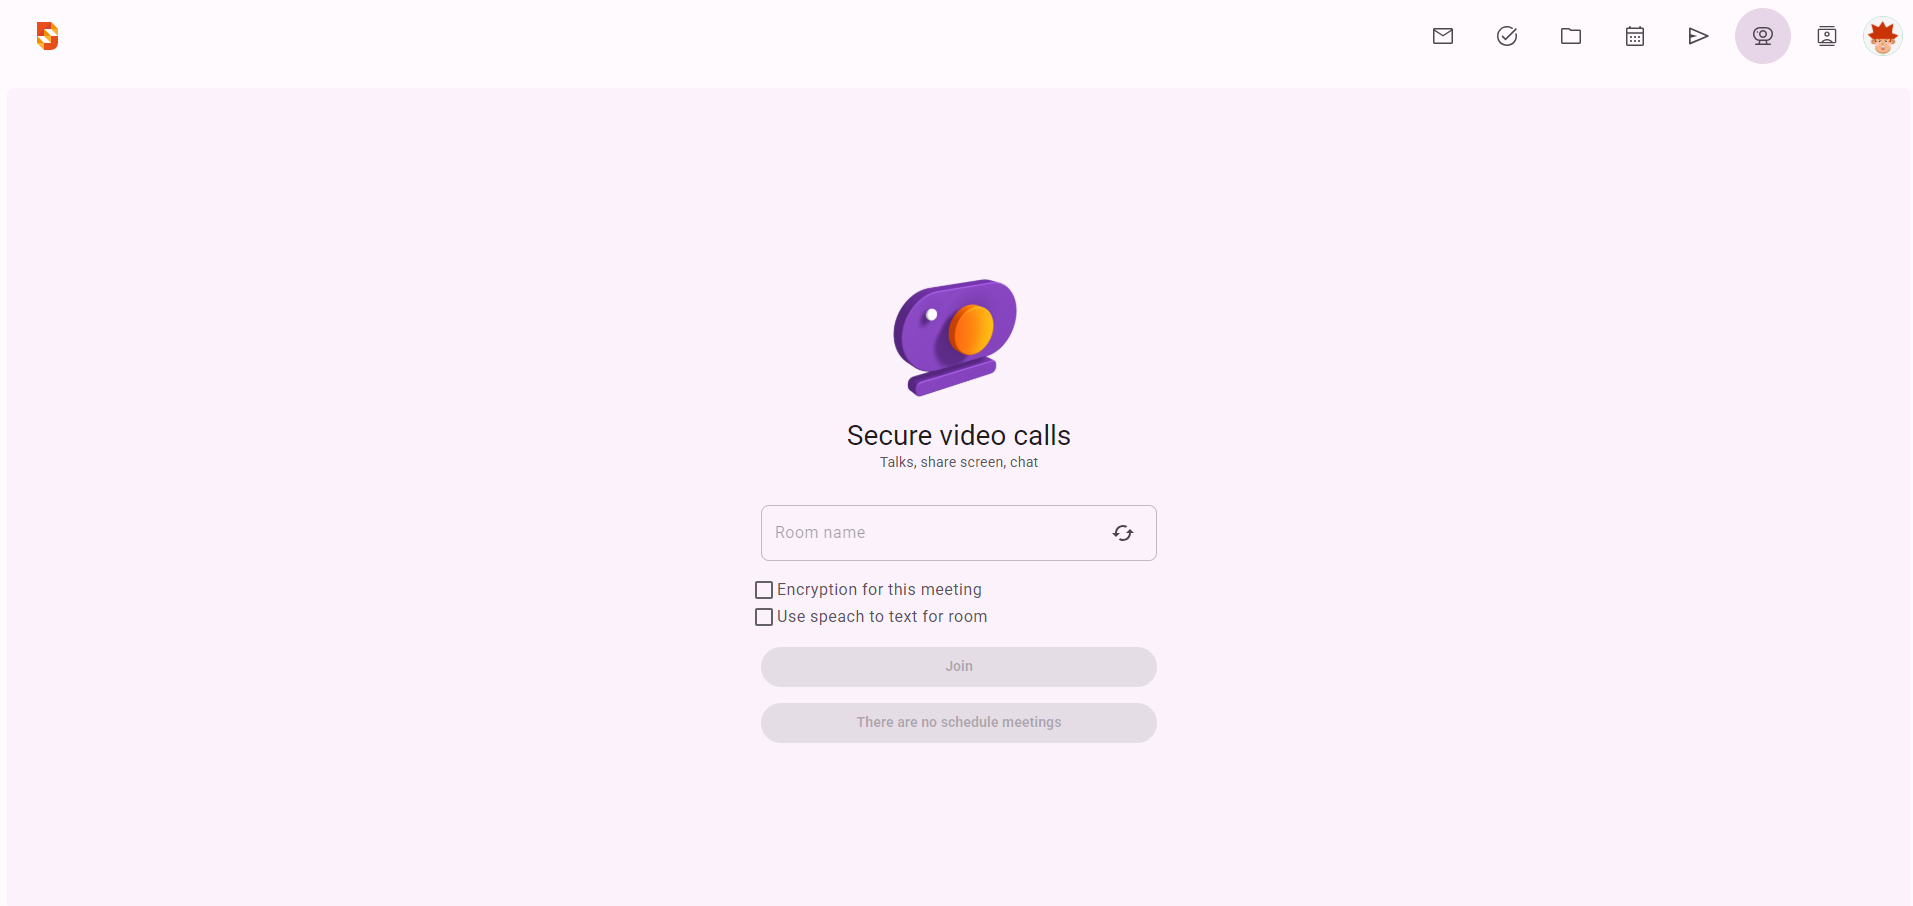
\includegraphics[width=1\linewidth]{images/вкс}
	\caption{Макет интерфейса сервиса <<Видеоконференцсвязь>>}
	\label{templ:image2}
\end{figure}

Макет интерфейса сервиса <<Календарь>> представлена на рисунке \ref{templ:image3} и состоит из:
\begin{itemize}
  \item компонента навигации по сервисам (1);
  \item кнопки для создания события (2);
  \item компонент уменьшенной версии календаря (3);
  \item кнопки фильтрации событий по типу (4);
  \item кнопки фильтрации событий по дате (5);
  \item окно для основной работы с календарём (6).
\end{itemize}
\begin{figure}[H]
	\centering
	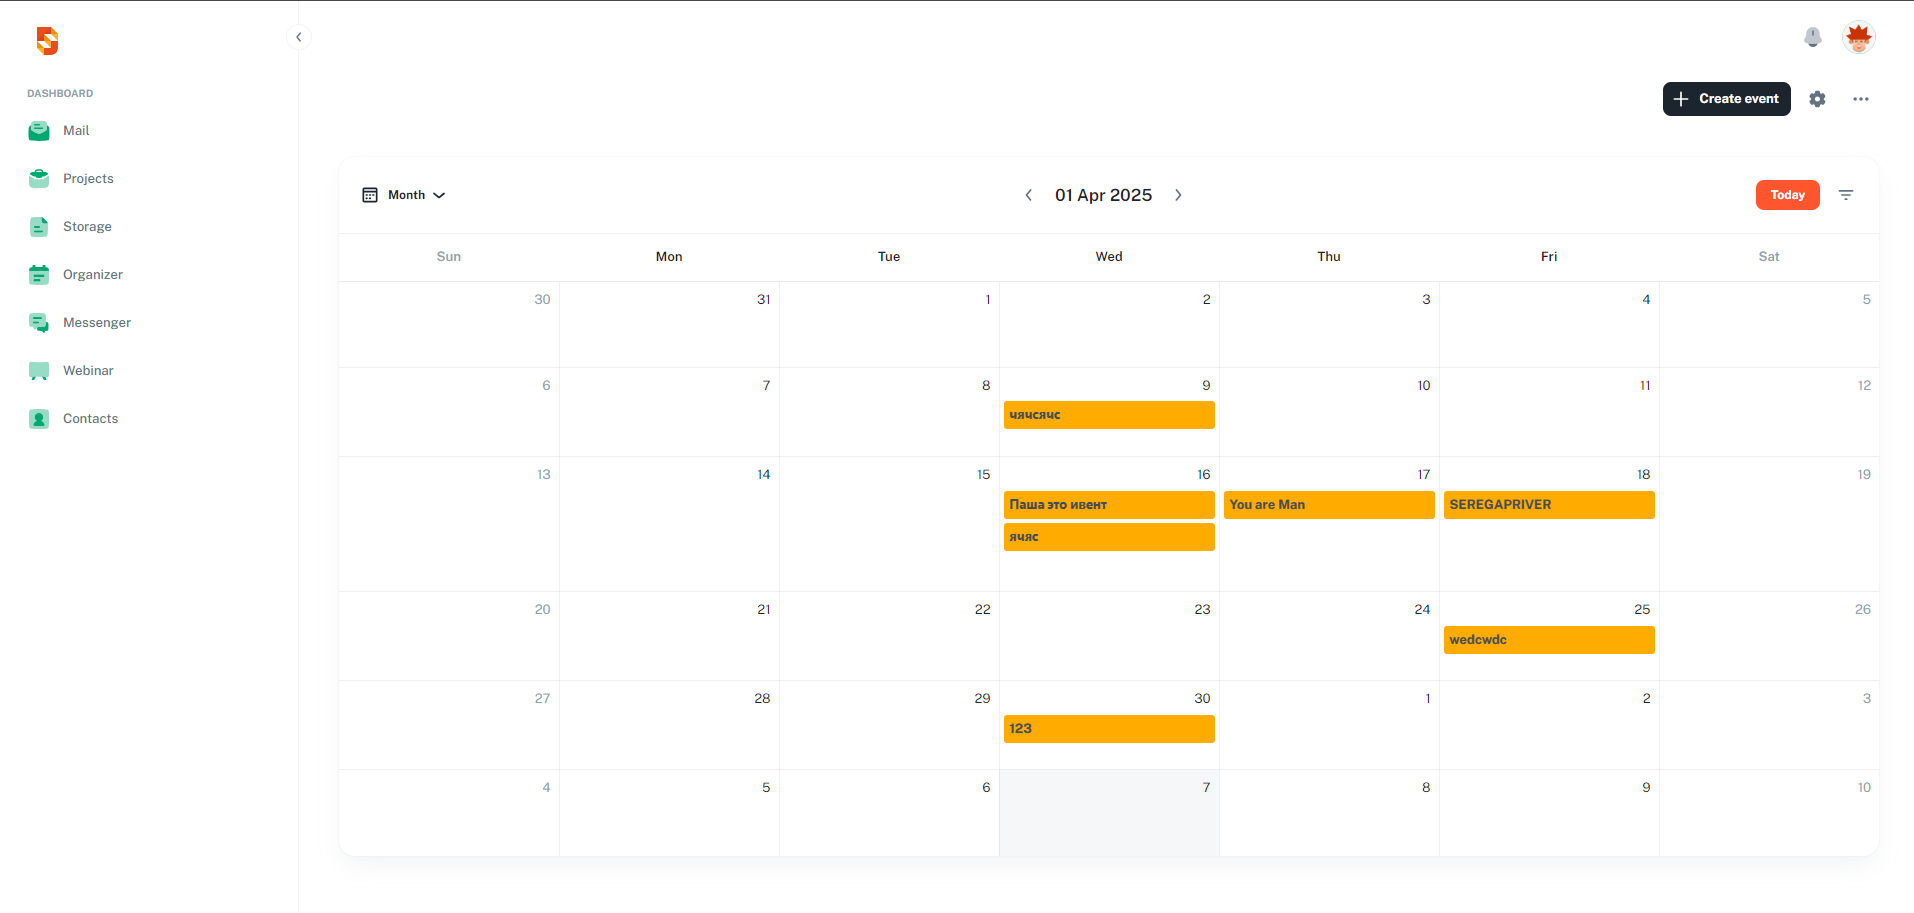
\includegraphics[width=1\linewidth]{images/календарь}
	\caption{Макет интерфейса сервиса <<Календарь>>}
	\label{templ:image3}
\end{figure}

Макет интерфейса создания события в сервисе <<Календарь>> представлена на рисунке \ref{templ:image3b} и состоит из:
\begin{itemize}
  \item всплывающего окна (1);
  \item кнопки для выбора категории (2);
  \item поля для ввода названия события (3);
  \item поля для ввода описания события (4);
  \item поля для ввода даты начала события и его параметров (5);
  \item поля для ввода названия видеоконференции (6);
  \item поля для выбора участников из сервиса <<Контакты>> (7).
\end{itemize}
\begin{figure}[H]
	\centering
	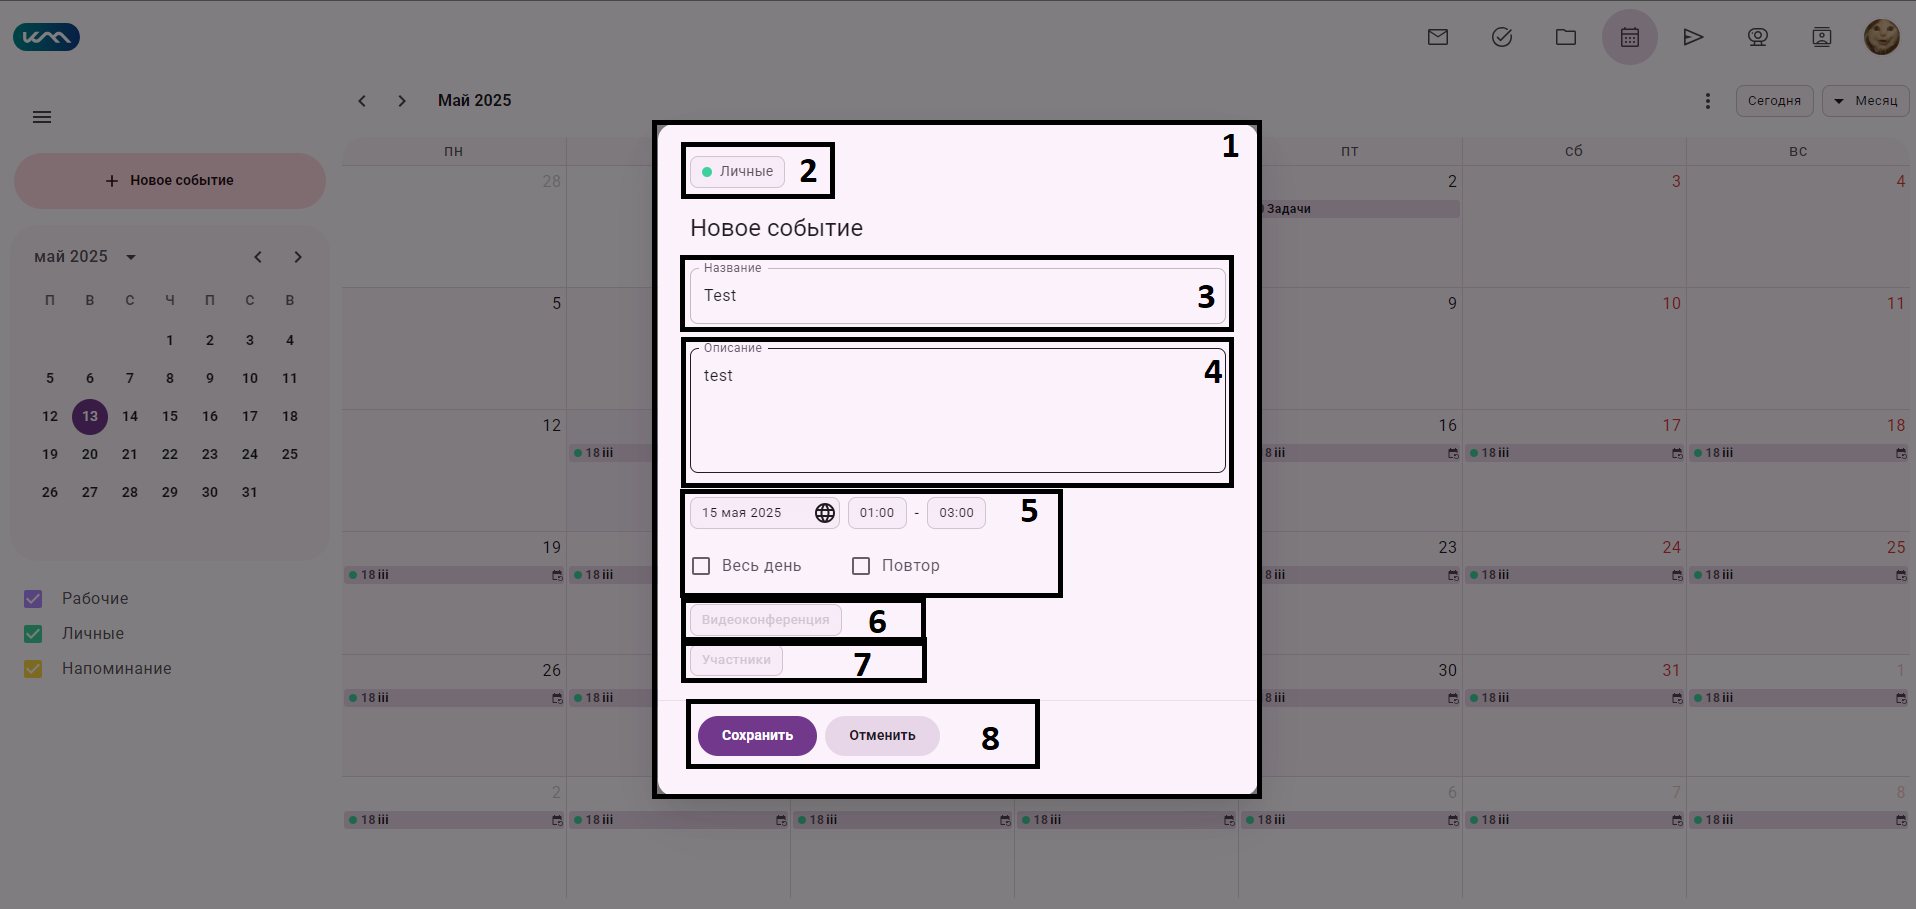
\includegraphics[width=1\linewidth]{images/календарь2}
	\caption{Макет интерфейса создания события}
	\label{templ:image3b}
\end{figure}

Макет интерфейса просмотра события в сервисе <<Календарь>> представлена на рисунке \ref{templ:image3c} и состоит из:
\begin{itemize}
  \item всплывающего окна (1);
  \item кнопок для редактирования, создания ссылки, удаления события (2);
  \item раздела с подробной информацией о событии (3);
  \item кнопок для подключения к ВКС, копирования события, прикрепления файла из сервиса <<Файлы>> (4);
  \item раздела с подробной информацией об участниках (5).
\end{itemize}
\begin{figure}[H]
	\centering
	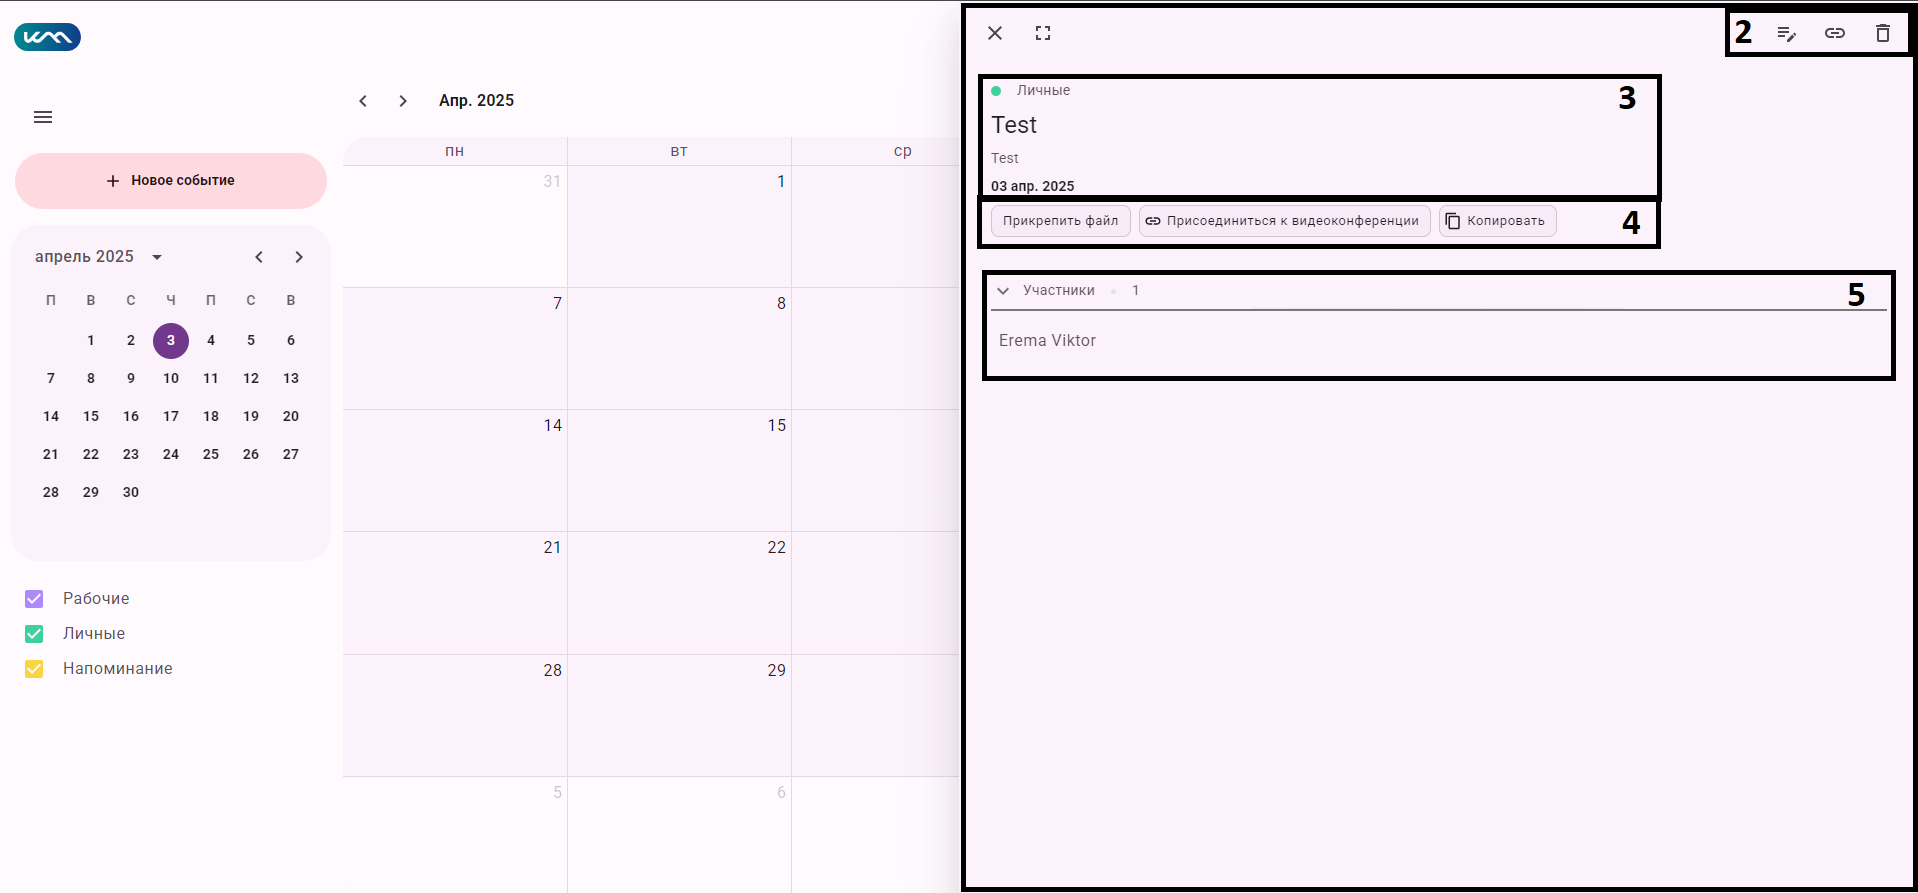
\includegraphics[width=1\linewidth]{images/календарь3}
	\caption{Макет интерфейса просмотра события}
	\label{templ:image3c}
\end{figure}

Макет интерфейса сервиса <<Панель управления>> представлена на рисунке \ref{templ:image4} и состоит из:
\begin{itemize}
  \item компонента навигации по сервисам (1);
  \item компонента "виджета" сервиса <<Почта>> (2);
  \item компонента "виджета" сервиса <<Проекты>> (3);
  \item компонента "виджета" сервиса <<Файлы>> (4);
  \item компонента "виджета" сервиса <<Календарь>> (5);
  \item компонента "виджета" сервиса <<Разговоры>> (6);
  \item компонента "виджета" сервиса <<Видеоконференцсвязь>> (7);
  \item компонента "виджета" сервиса <<Контакты>> (8).
\end{itemize}
\begin{figure}[H]
	\centering
	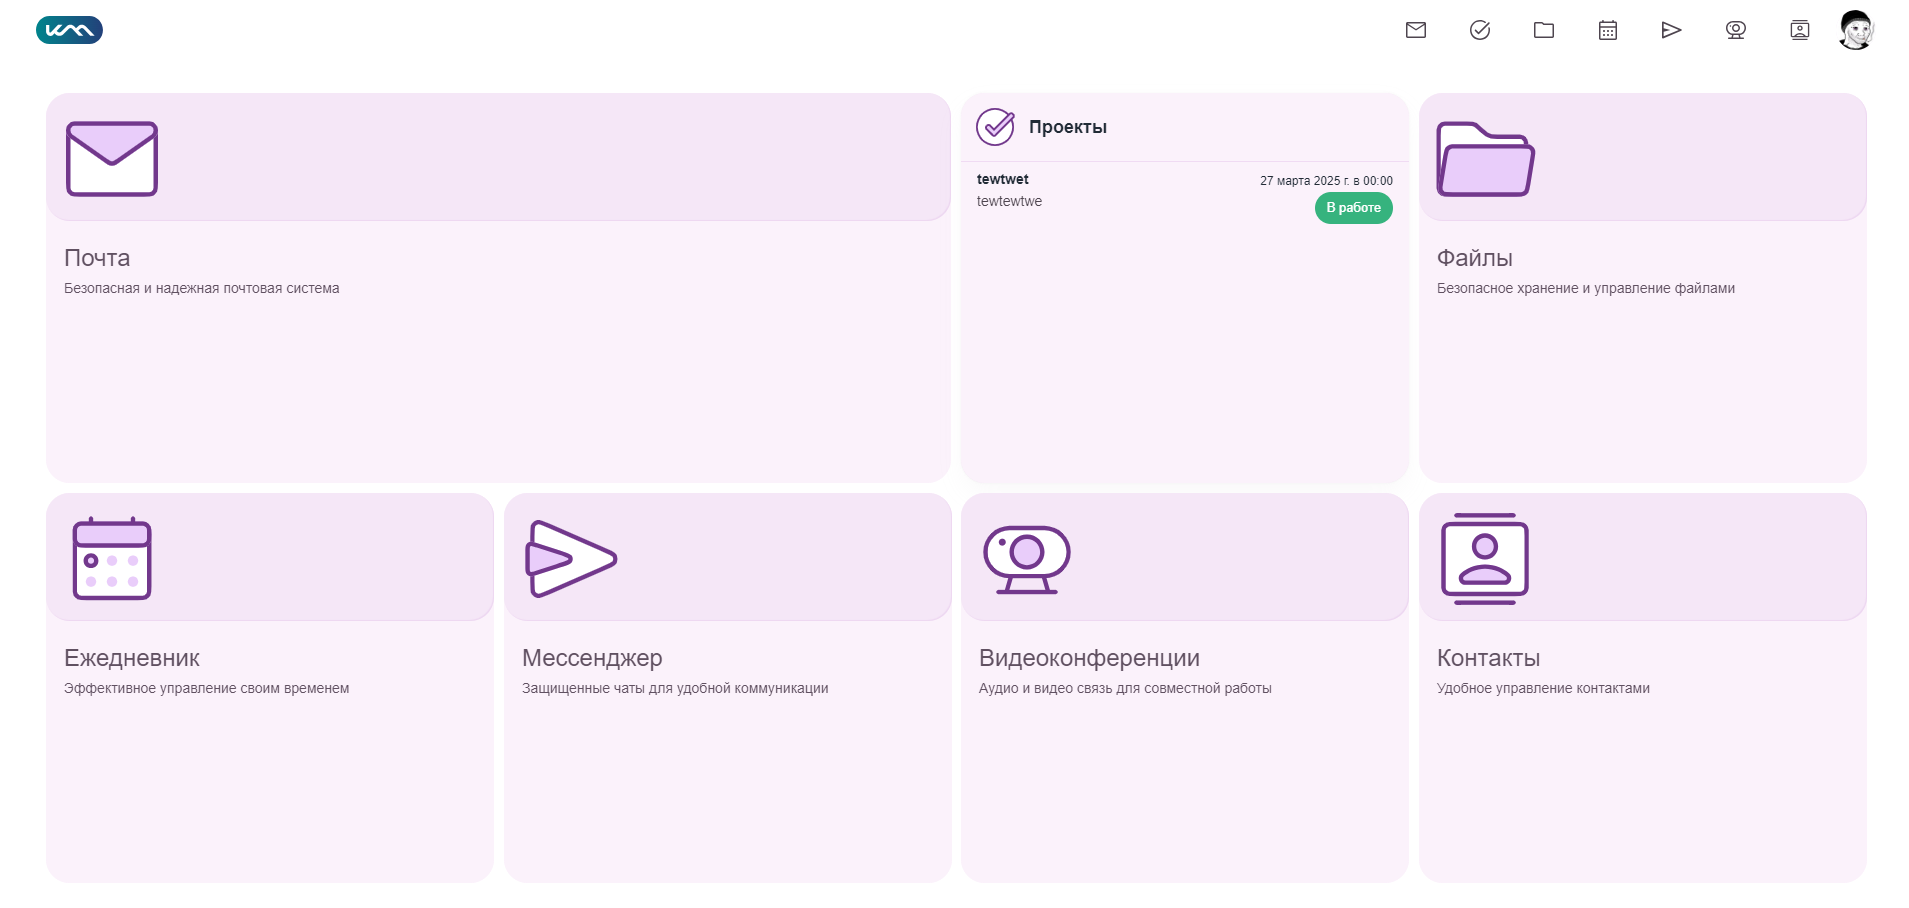
\includegraphics[width=1\linewidth]{images/дашборд}
	\caption{Макет интерфейса сервиса <<Панель управления>>}
	\label{templ:image4}
\end{figure}

Макет интерфейса сервиса <<Контакты>> представлена на рисунке \ref{templ:image5} и состоит из:
\begin{itemize}
  \item компонента навигации по сервисам (1);
  \item кнопки для создания контакта (2);
  \item списка папок (3);
  \item окна для работы с контактами (4);
  \item компонента пагинации (5).
\end{itemize}
\begin{figure}[H]
	\centering
	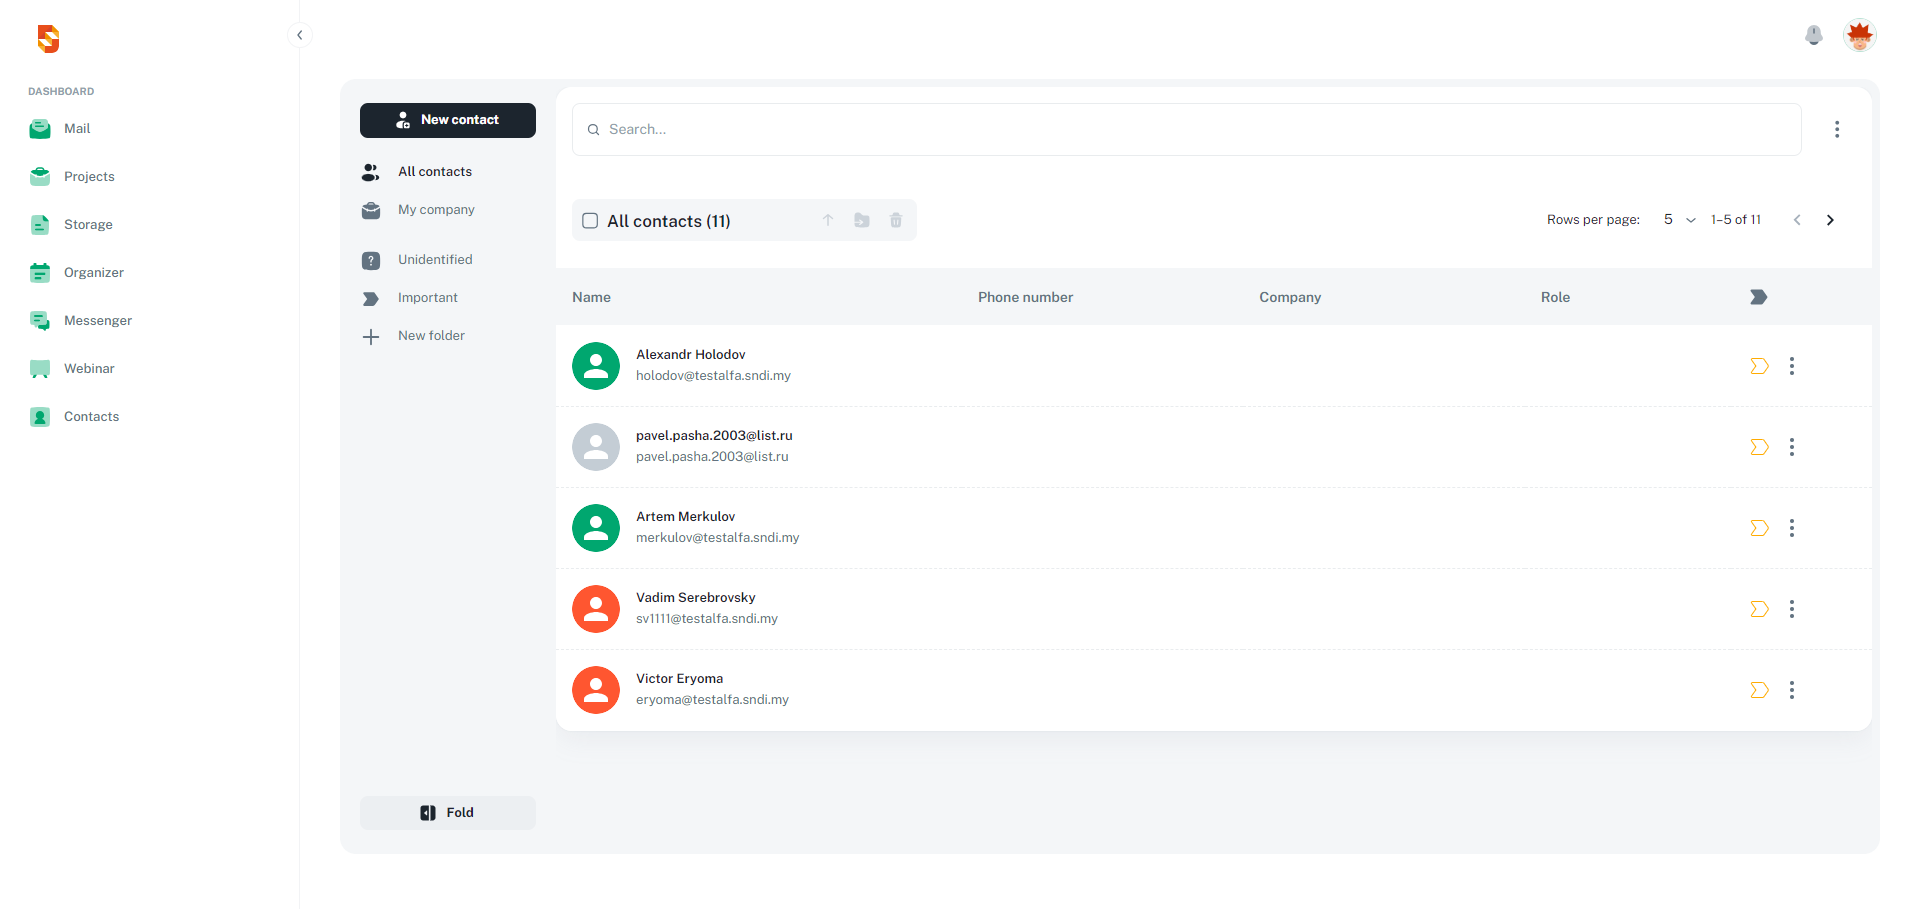
\includegraphics[width=1\linewidth]{images/контакты}
	\caption{Макет интерфейса сервиса <<Контакты>>}
	\label{templ:image5}
\end{figure}

Макет интерфейса создания контакта в сервисе <<Контакты>> представлена на рисунке \ref{templ:image5b} и состоит из:
\begin{itemize}
  \item всплывающего окна (1);
  \item поля для ввода имени (2);
  \item поля для ввода фамилии (3);
  \item поля для ввода даты рождения (4);
  \item поля для ввода компании (5);
  \item поля для ввода должности (6);
  \item поля для ввода почты (7);
  \item поля для ввода телефона (8);
  \item кнопок действий (9).
\end{itemize}
\begin{figure}[H]
	\centering
	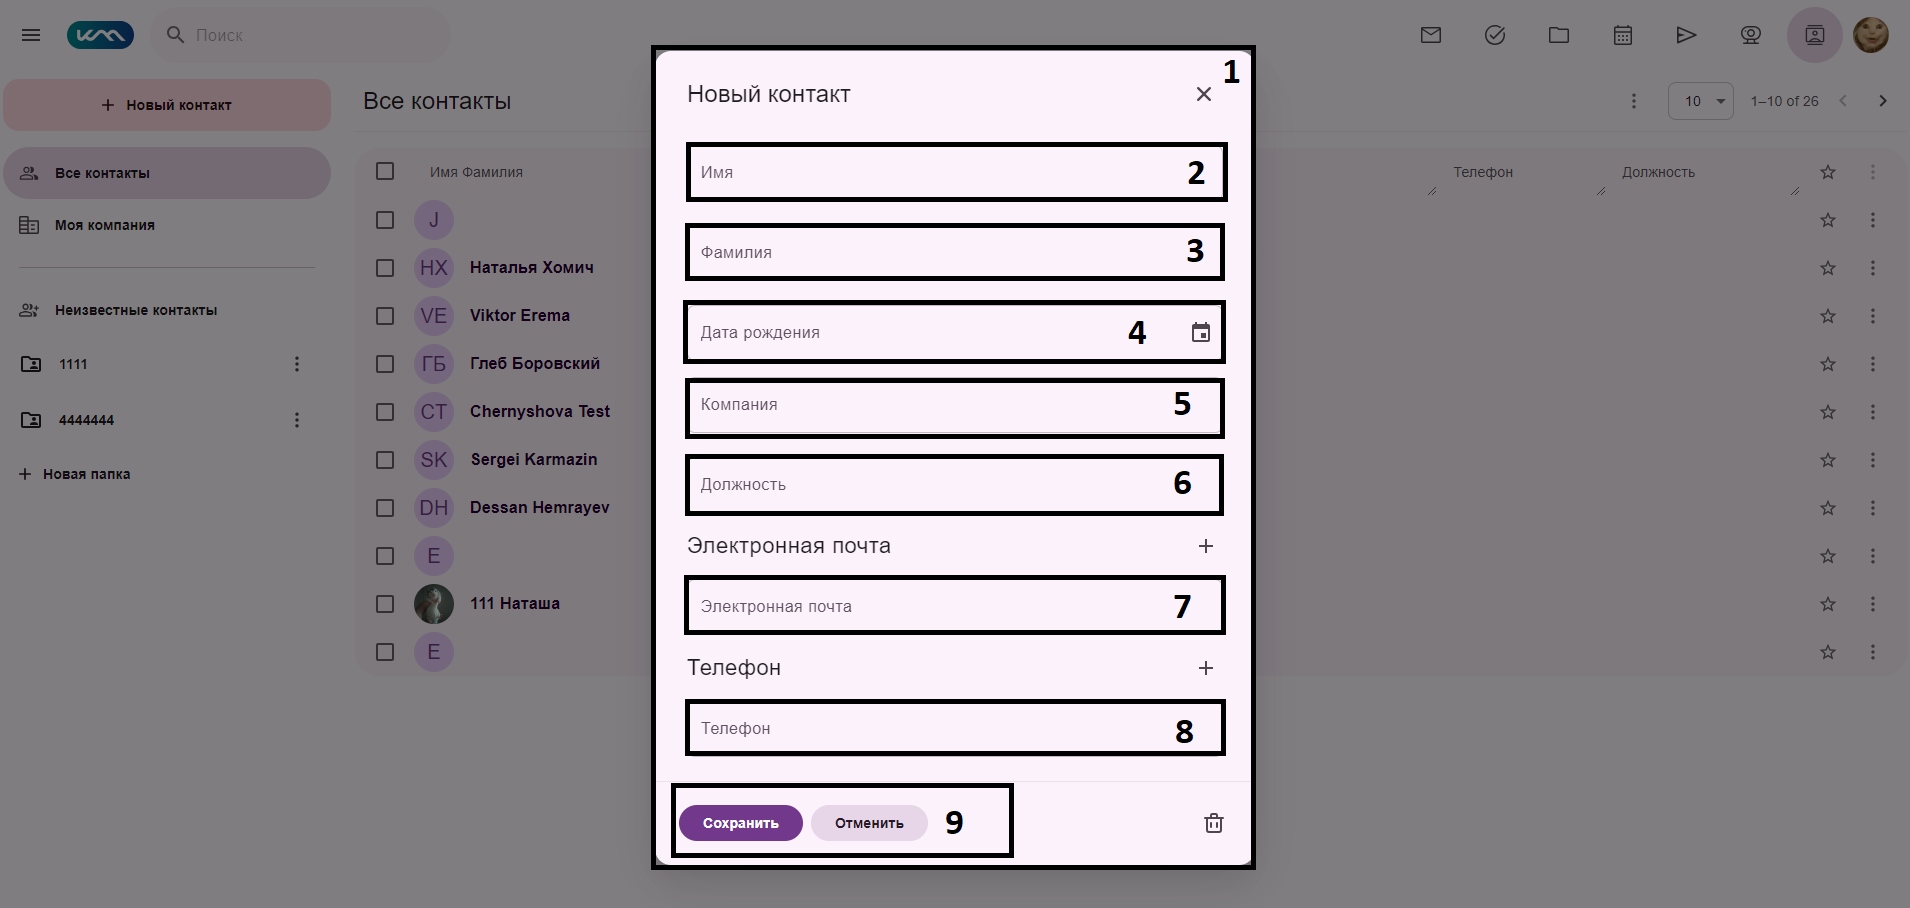
\includegraphics[width=1\linewidth]{images/контакты2}
	\caption{Макет интерфейса создания контакта}
	\label{templ:image5b}
\end{figure}

Макет интерфейса просмотра контакта в сервисе <<Контакты>> представлена на рисунке \ref{templ:image5b} и состоит из:
\begin{itemize}
  \item окна с информацией о контакте (1);
  \item кнопок для скачивания, редактирования, удаления и отправки контакта (2);
  \item кнопки для написания письма этому человеку в сервисе <<Почта>> (3);
  \item окна с подробной информацией о контакте (4).
\end{itemize}
\begin{figure}[H]
	\centering
	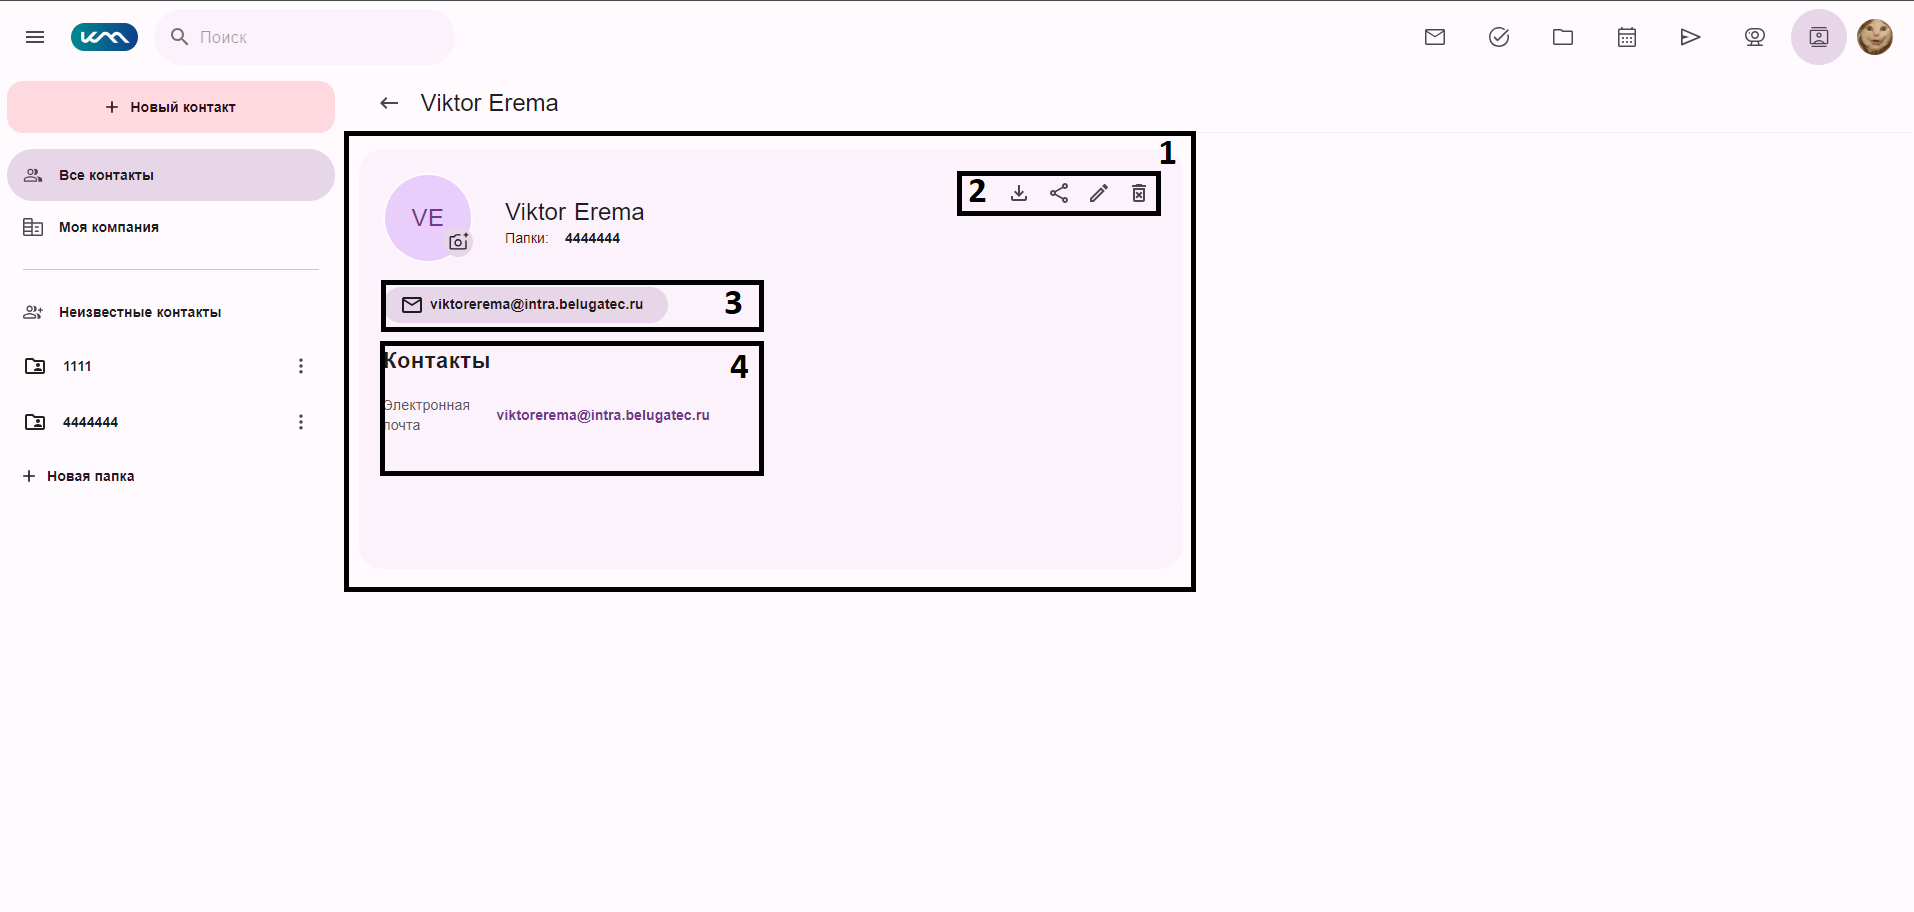
\includegraphics[width=1\linewidth]{images/контакты3}
	\caption{Макет интерфейса просмотра контакта}
	\label{templ:image5b}
\end{figure}

Макет интерфейса создания папки в сервисе <<Контакты>> представлена на рисунке \ref{templ:image5c} и состоит из:
\begin{itemize}
  \item всплывающего окна (1);
  \item поля для ввода названия папки (2);
  \item кнопок действий (3).
\end{itemize}
\begin{figure}[H]
	\centering
	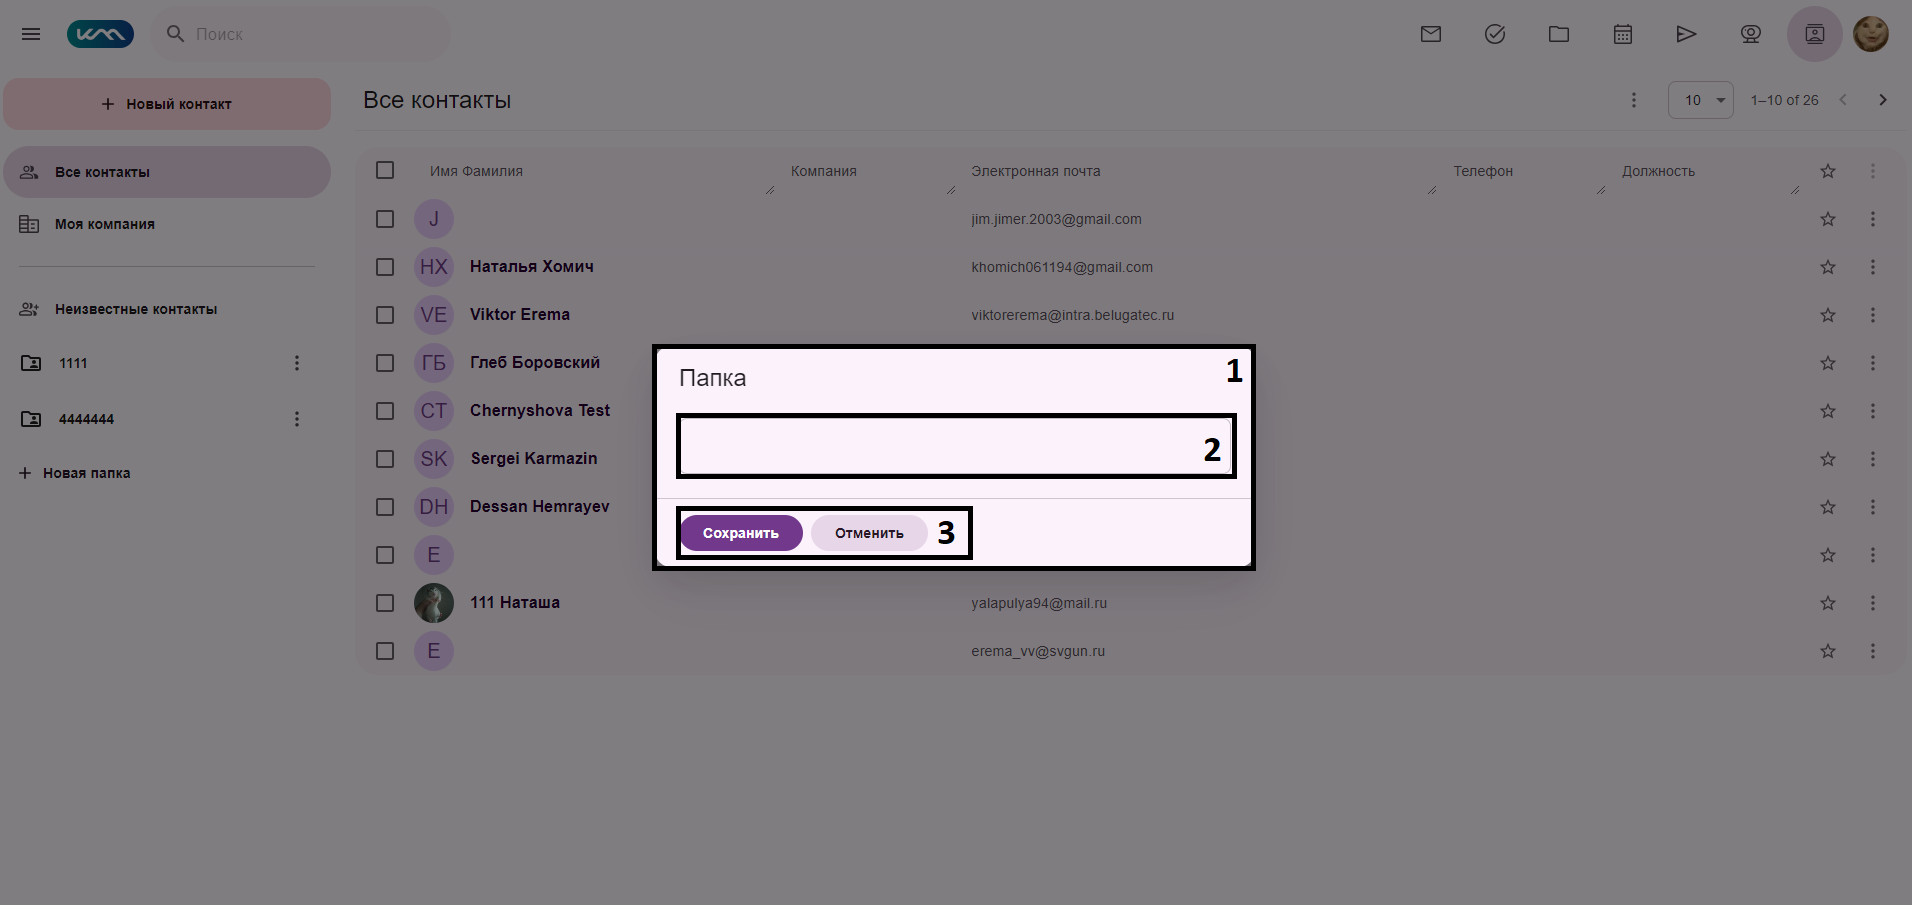
\includegraphics[width=1\linewidth]{images/контакты4}
	\caption{Макет интерфейса создания папки}
	\label{templ:image5c}
\end{figure}

Макет интерфейса сервиса <<Настройки>> представлена на рисунке \ref{templ:image6} и состоит из:
\begin{itemize}
  \item компонента навигации по сервисам (1);
  \item компонента навигации по разделам (2);
  \item кнопки для выхода из учётной записи (3);
  \item раздела смены темы (4);
  \item раздела смены цветовой палитры (5);
  \item раздела редактирования подписи электронной почты (6).
\end{itemize}
\begin{figure}[H]
	\centering
	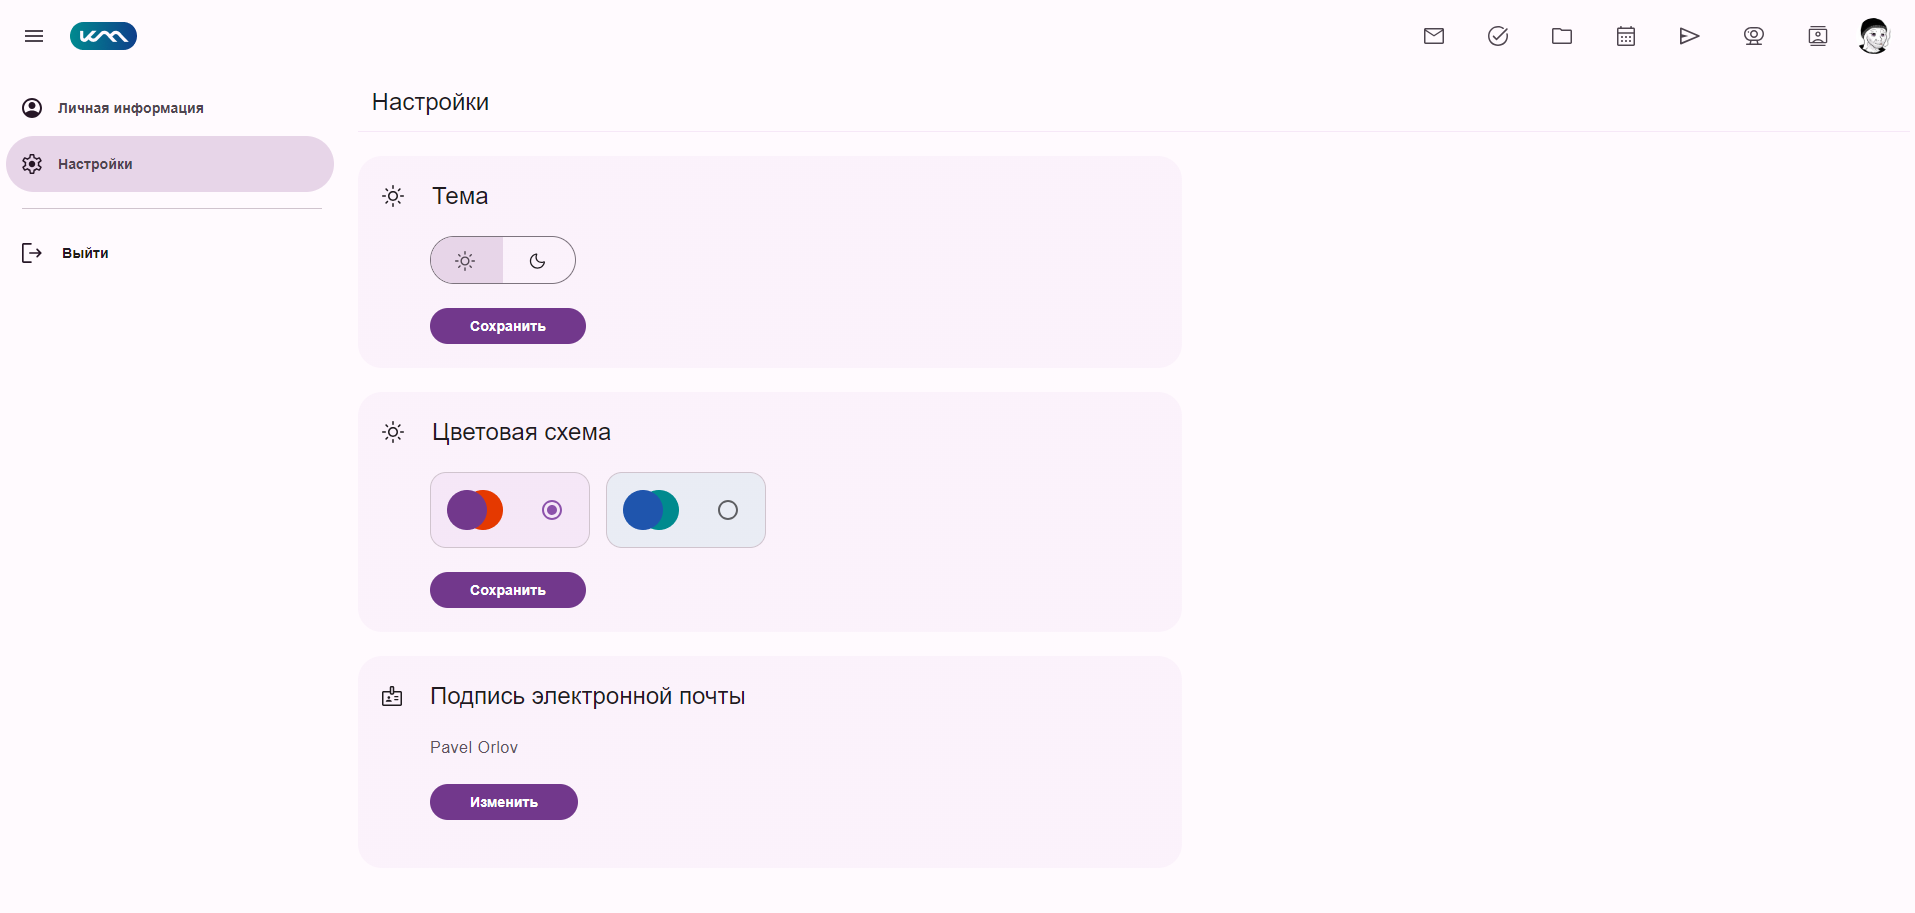
\includegraphics[width=1\linewidth]{images/настройки}
	\caption{Макет интерфейса сервиса <<Настройки>>}
	\label{templ:image6}
\end{figure}

Макет интерфейса изменения цифровой подписи в сервисе <<Настройки>> представлена на рисунке \ref{templ:image6b} и состоит из:
\begin{itemize}
  \item всплывающего окна (1);
  \item поля для ввода цифровой подписи (2);
  \item кнопок действий (3).
\end{itemize}
\begin{figure}[H]
	\centering
	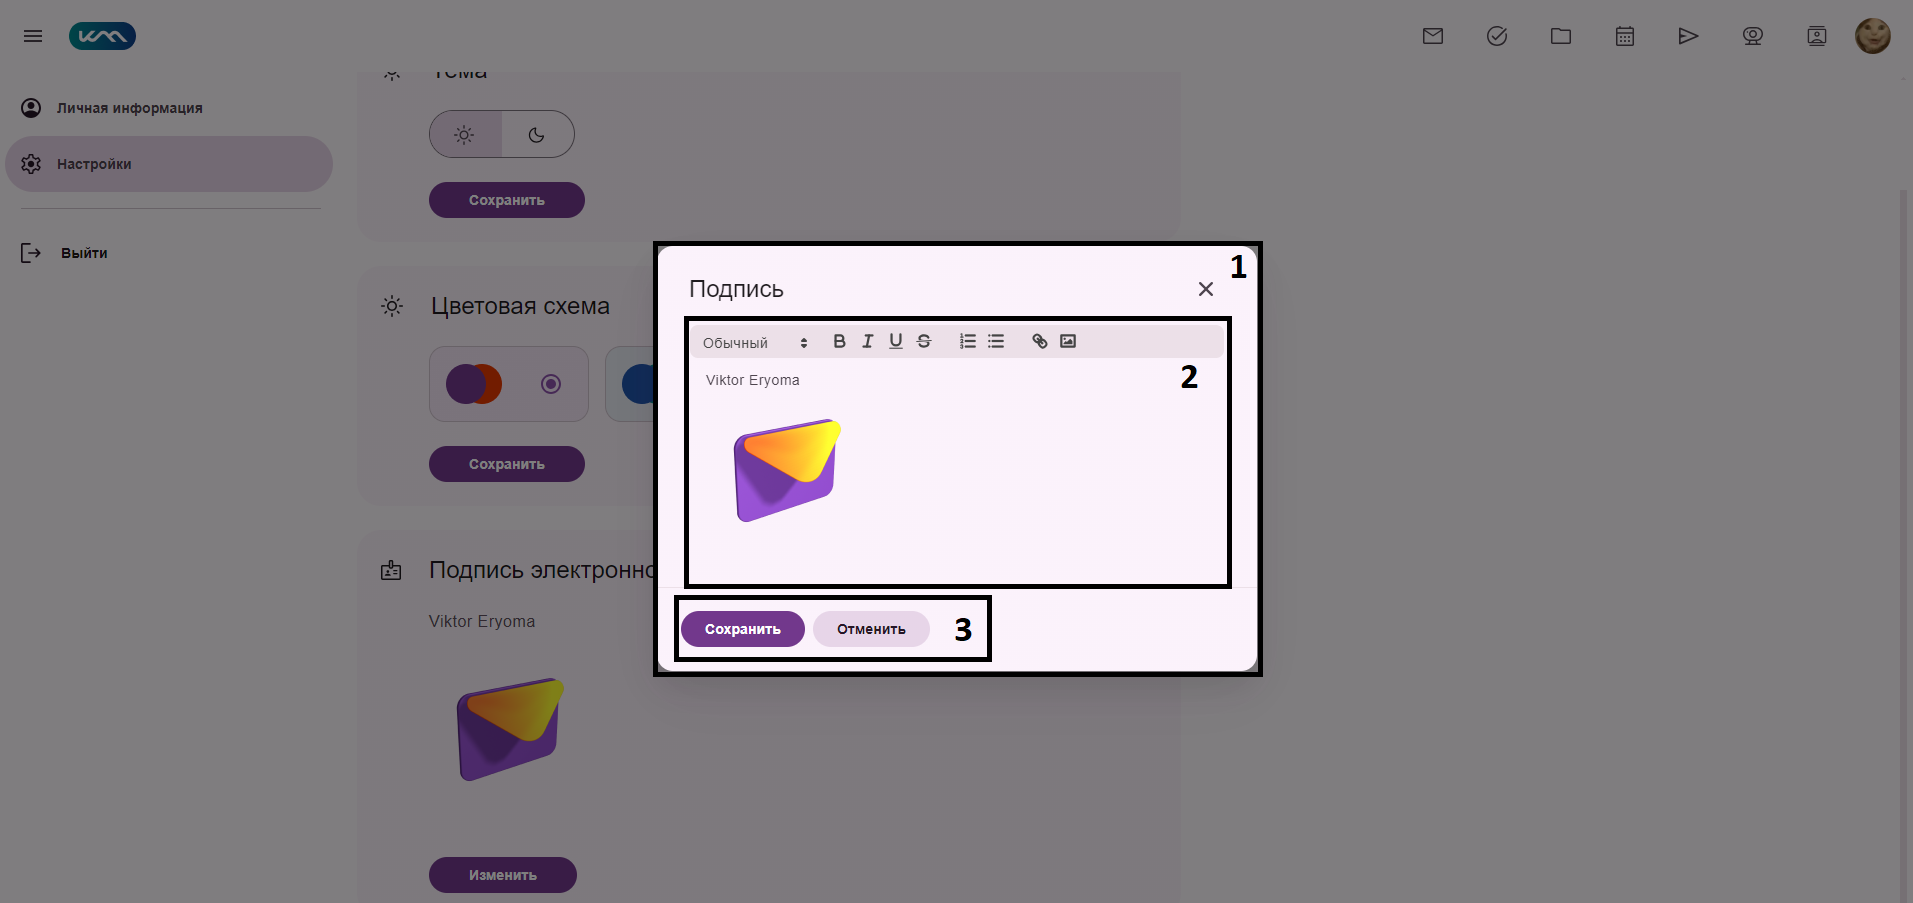
\includegraphics[width=1\linewidth]{images/настройки2}
	\caption{Макет интерфейса изменения цифровой подписи}
	\label{templ:image6b}
\end{figure}

Макет интерфейса сервиса <<Проекты>> представлена на рисунке \ref{templ:image7} и состоит из:
\begin{itemize}
  \item компонента навигации по сервисам (1);
  \item кнопки для создания раздела (2);
  \item компонента навигации по разделам (3);
  \item окна для работы с задачами (4);
  \item кнопки для создания задачи (5).
\end{itemize}
\begin{figure}[H]
	\centering
	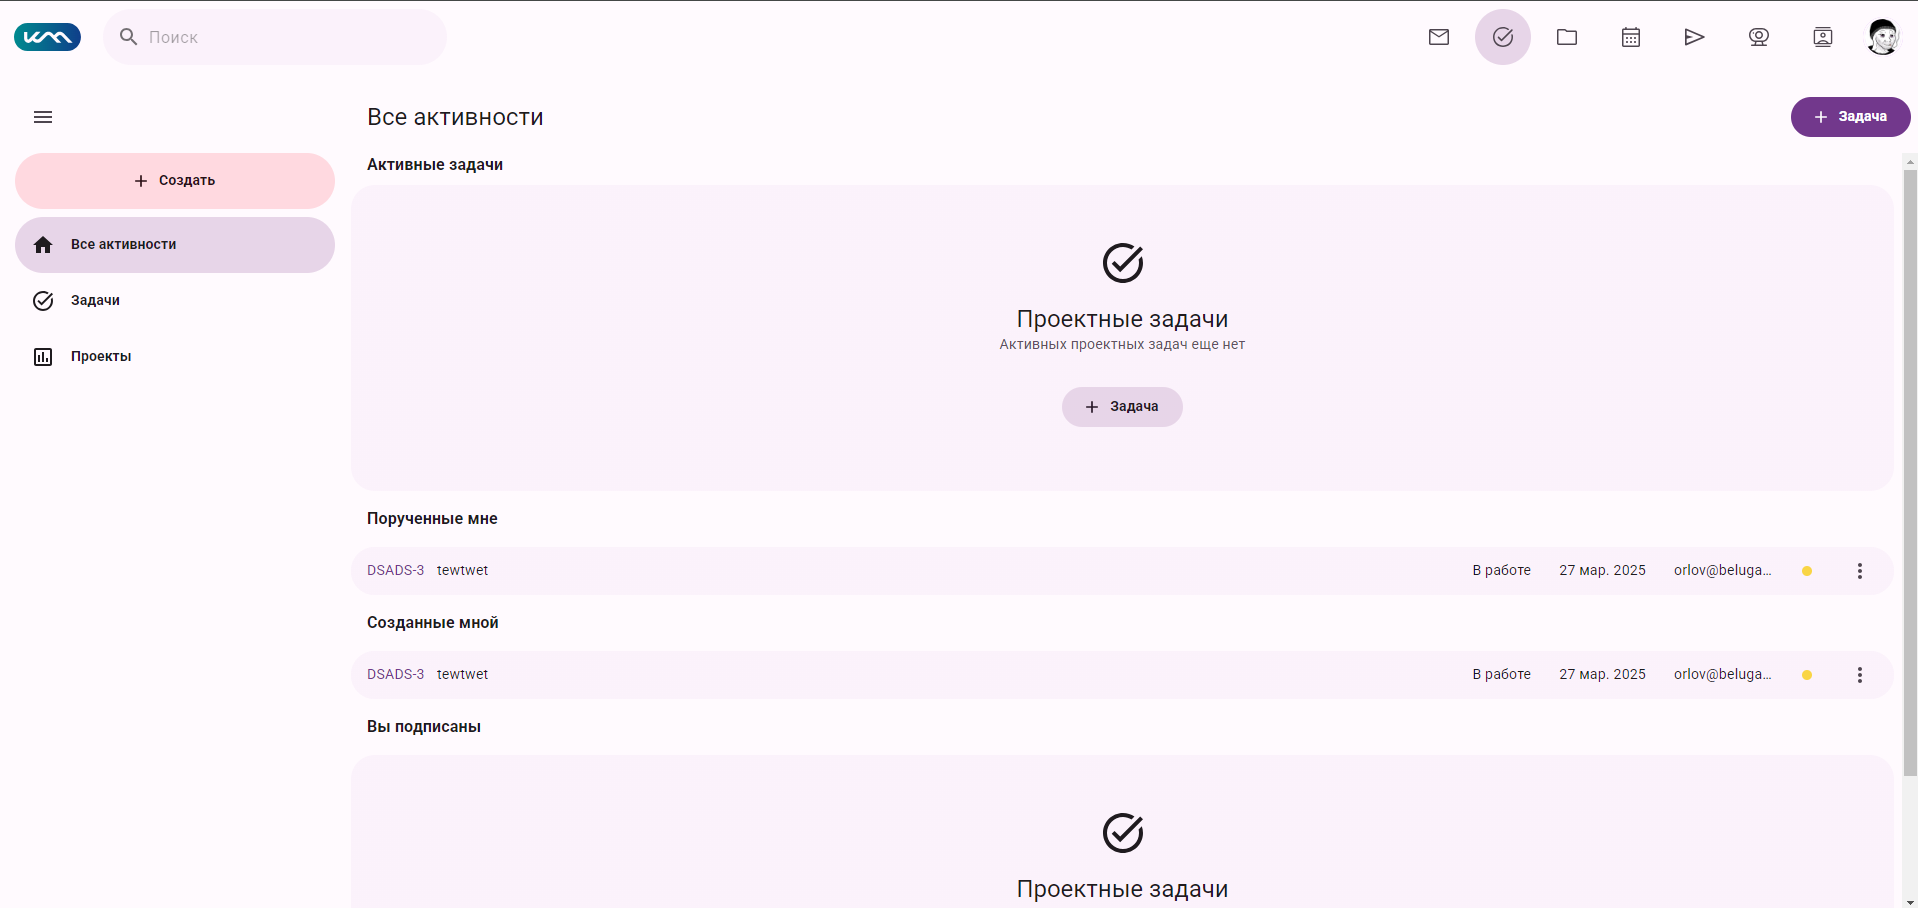
\includegraphics[width=1\linewidth]{images/проекты}
	\caption{Макет интерфейса сервиса <<Проекты>>}
	\label{templ:image7}
\end{figure}

Макет интерфейса создания проекта в сервисе <<Проекты>> представлена на рисунке \ref{templ:image7b} и состоит из:
\begin{itemize}
  \item всплывающего окна (1);
  \item поля для ввода названия проекта (2);
  \item поля для ввода описания проекта (3);
  \item кнопок действий (4).
\end{itemize}
\begin{figure}[H]
	\centering
	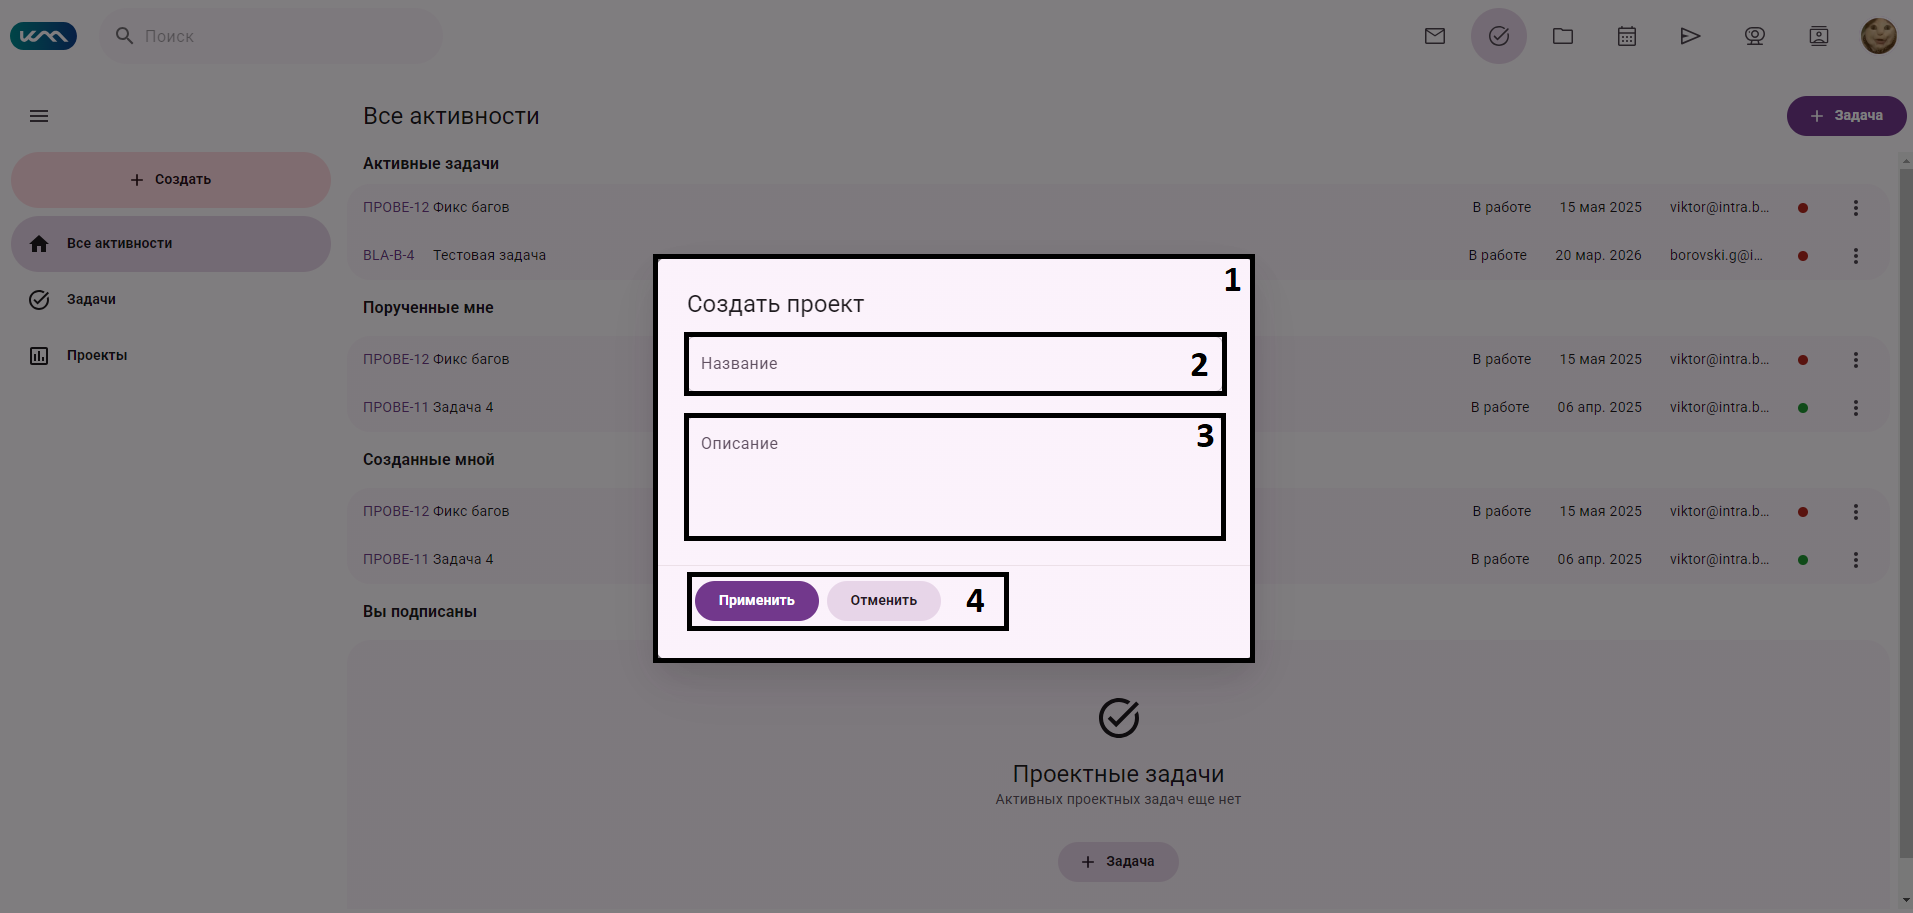
\includegraphics[width=1\linewidth]{images/проекты2}
	\caption{Макет интерфейса создания проекта}
	\label{templ:image7b}
\end{figure}

Макет интерфейса создания задачи в сервисе <<Проекты>> представлена на рисунке \ref{templ:image7c} и состоит из:
\begin{itemize}
  \item всплывающего окна (1);
  \item кнопки для выбора проекта (2);
  \item поля для ввода названия задачи (3);
  \item поля для ввода описания задачи (4);
  \item кнопок для выбора даты начала/конца задачи, приоритета, исполнителя (5);
  \item кнопок действий (6).
\end{itemize}
\begin{figure}[H]
	\centering
	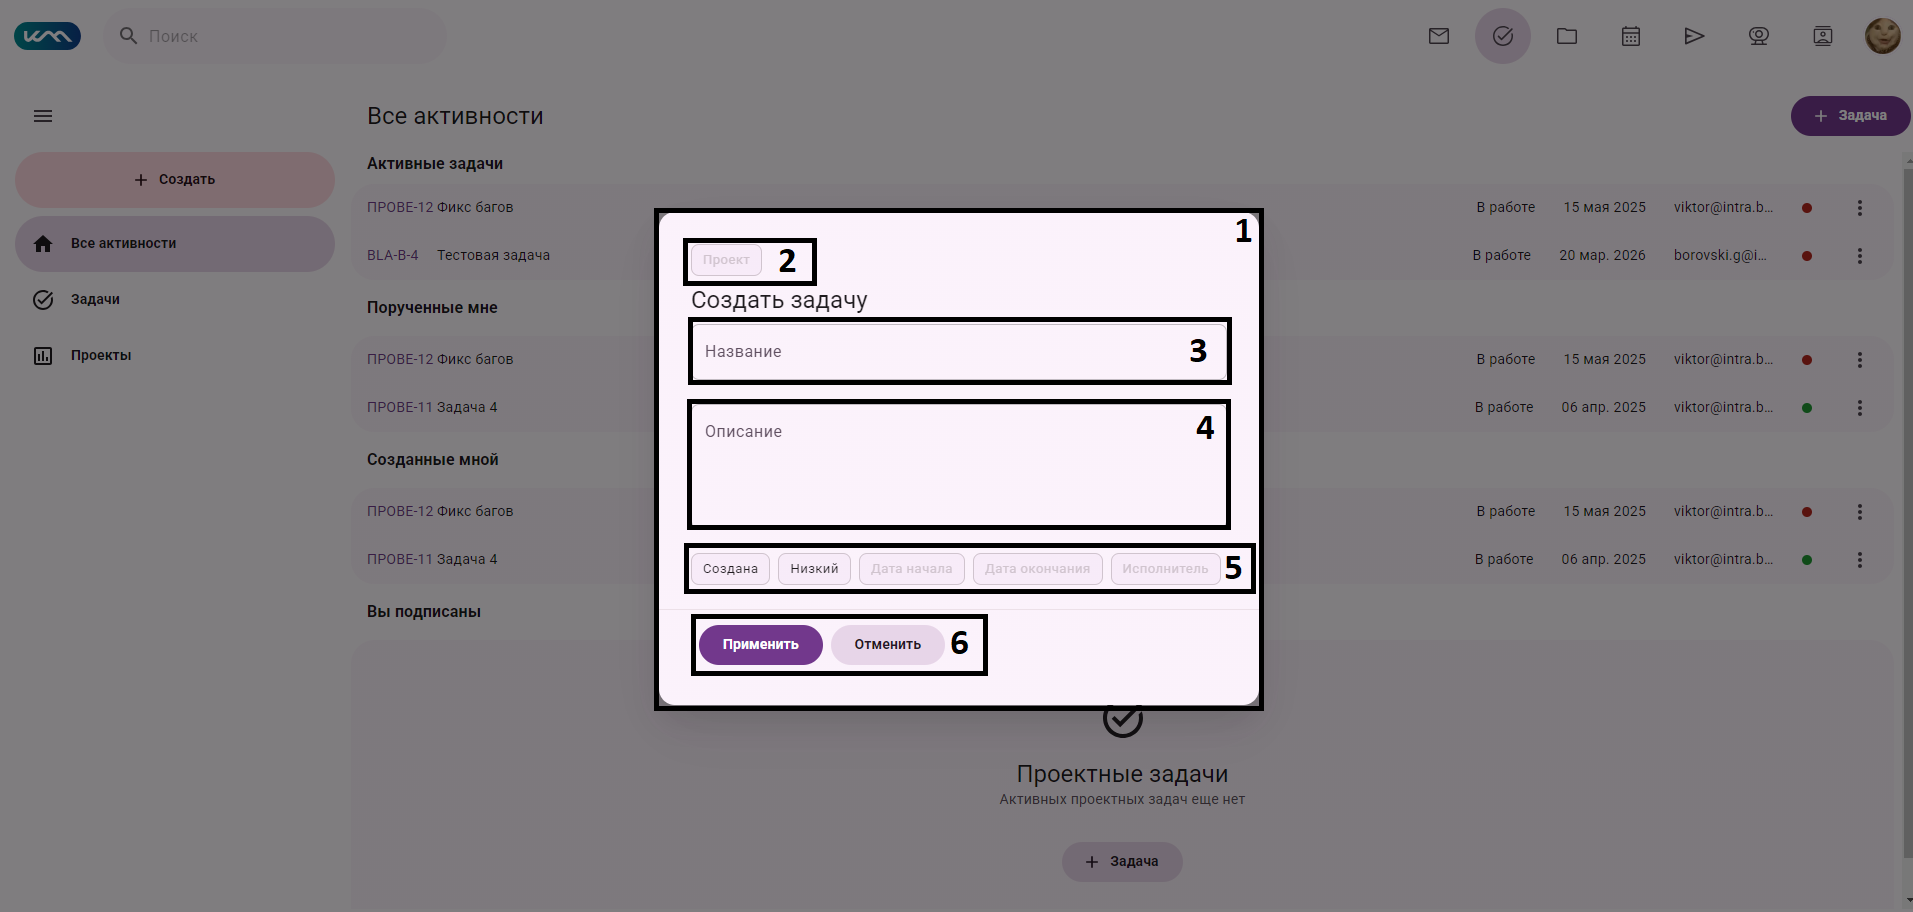
\includegraphics[width=1\linewidth]{images/проекты3}
	\caption{Макет интерфейса создания задачи}
	\label{templ:image7c}
\end{figure}

Макет интерфейса просмотра задачи в сервисе <<Проекты>> представлена на рисунке \ref{templ:image7d} и состоит из:
\begin{itemize}
  \item всплывающего окна (1);
  \item кнопок для отслеживания, удаления и архивирования задачи (2);
  \item подробной информации о задаче (3);
  \item кнопок для прикрепления файлов/ссылок, добавление подзадачи (4);
  \item раздела с комментариями (5);
  \item поля для ввода комментария (6);
  \item кнопки для отправки комментария (7).
\end{itemize}
\begin{figure}[H]
	\centering
	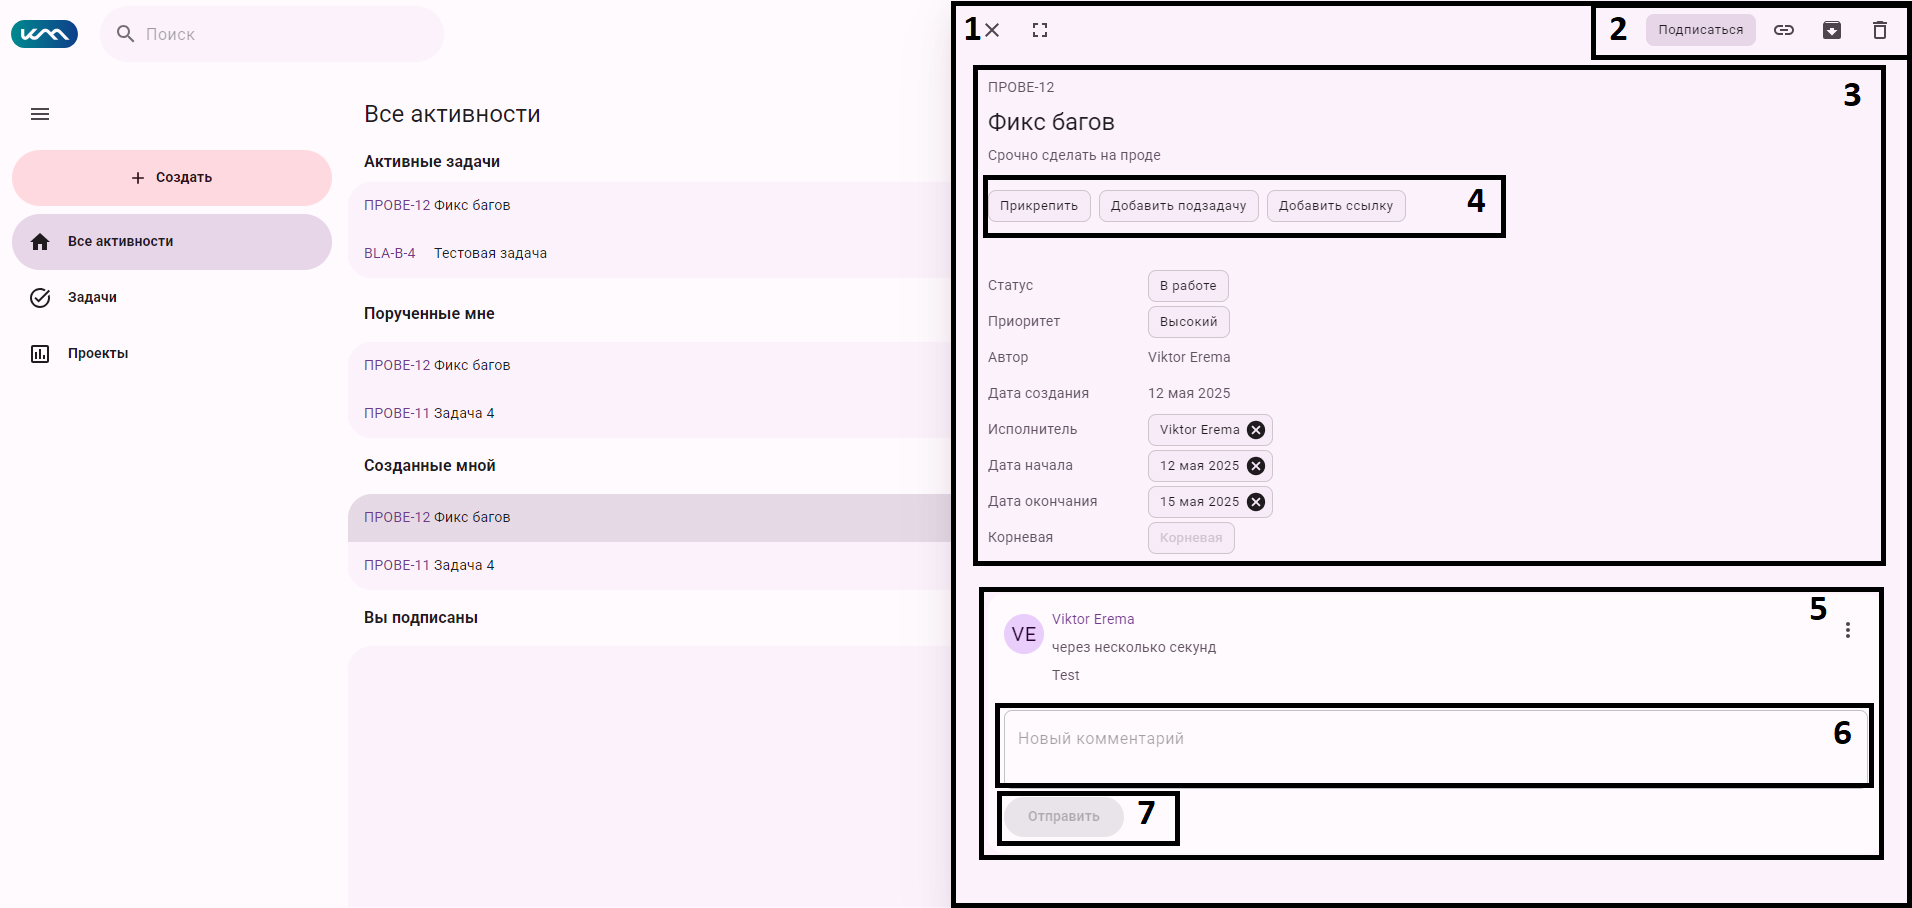
\includegraphics[width=1\linewidth]{images/проекты4}
	\caption{Макет интерфейса просмотра задачи}
	\label{templ:image7d}
\end{figure}

Макет интерфейса сервиса <<Разговоры>> представлена на рисунке \ref{templ:image8} и состоит из:
\begin{itemize}
  \item компонента навигации по сервисам (1);
  \item кнопки для создания комнаты (2);
  \item списка комнат (3);
  \item кнопки для создания диалога (4);
  \item кнопки для создания канала (5);
  \item окна для работы с комнатой (6);
  \item поля для написания сообщения (7).
\end{itemize}
\begin{figure}[H]
	\centering
	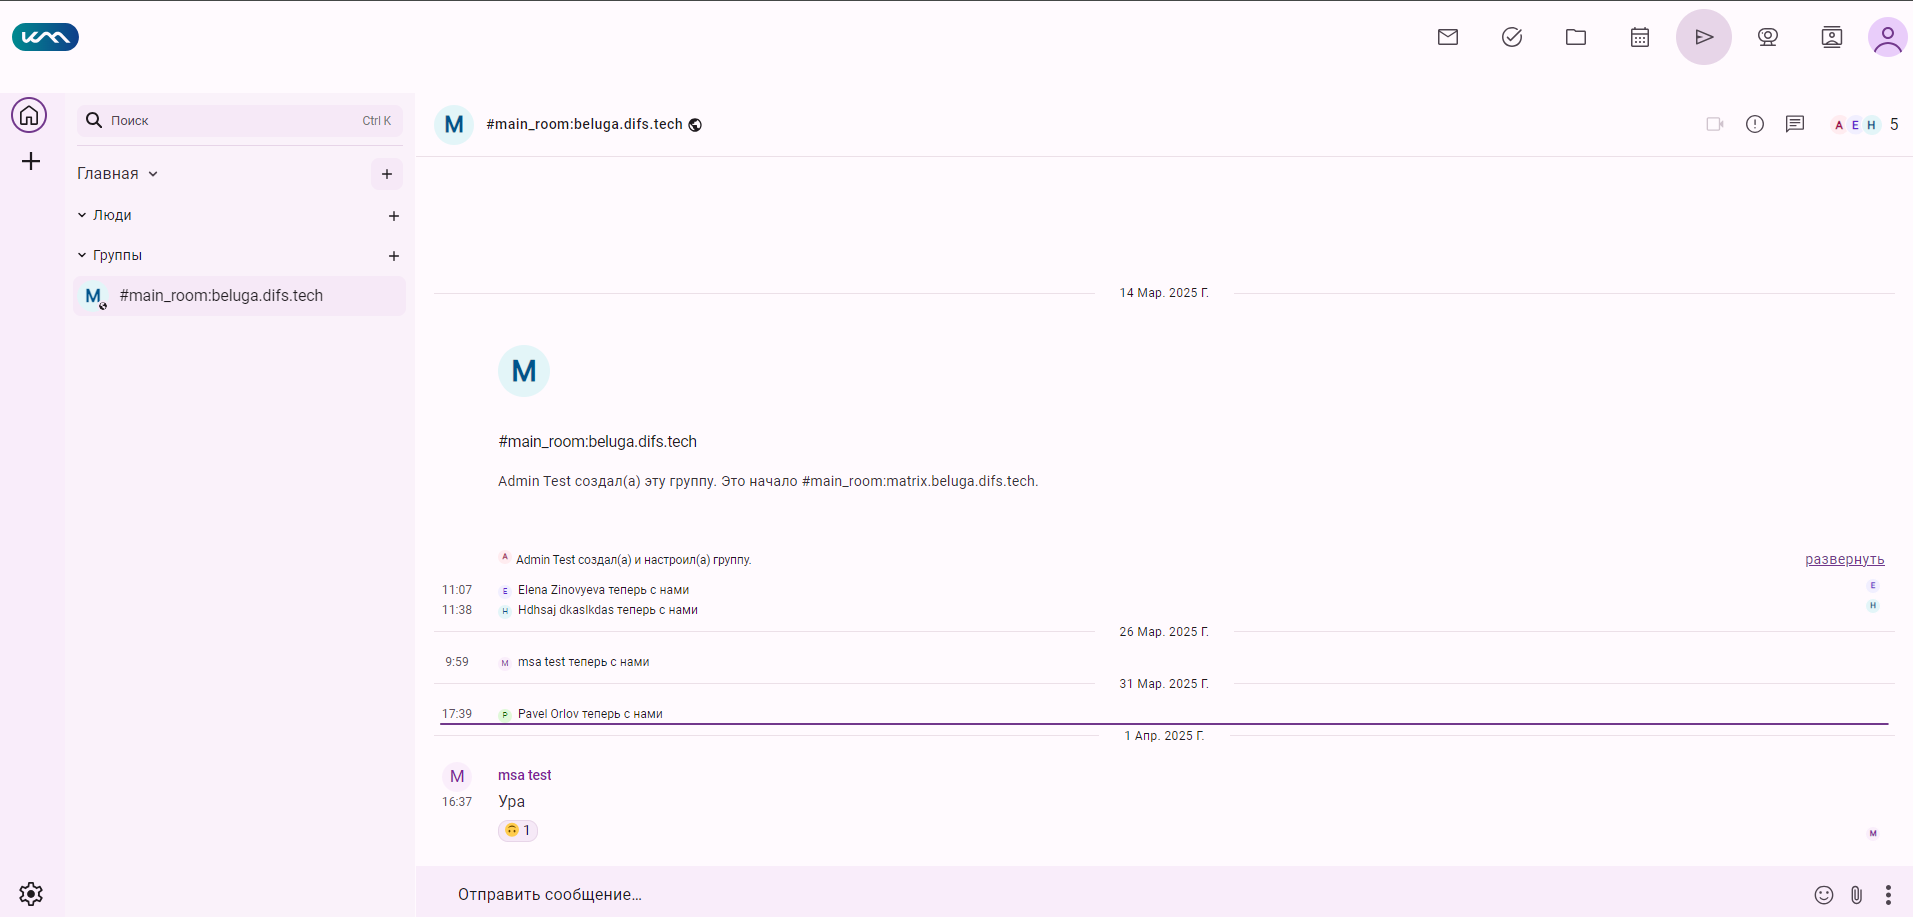
\includegraphics[width=1\linewidth]{images/разговоры}
	\caption{Макет интерфейса сервиса <<Разговоры>>}
	\label{templ:image8}
\end{figure}

Макет интерфейса сервиса <<Файлы>> представлена на рисунке \ref{templ:image9} и состоит из:
\begin{itemize}
  \item компонента навигации по сервисам (1);
  \item кнопки для создания папки/загрузки файла в текущую папку (2);
  \item списка папок (3);
  \item окна для работы с файлами (4);
  \item кнопки для перехода в настройки сервиса (5).
\end{itemize}
\begin{figure}[H]
	\centering
	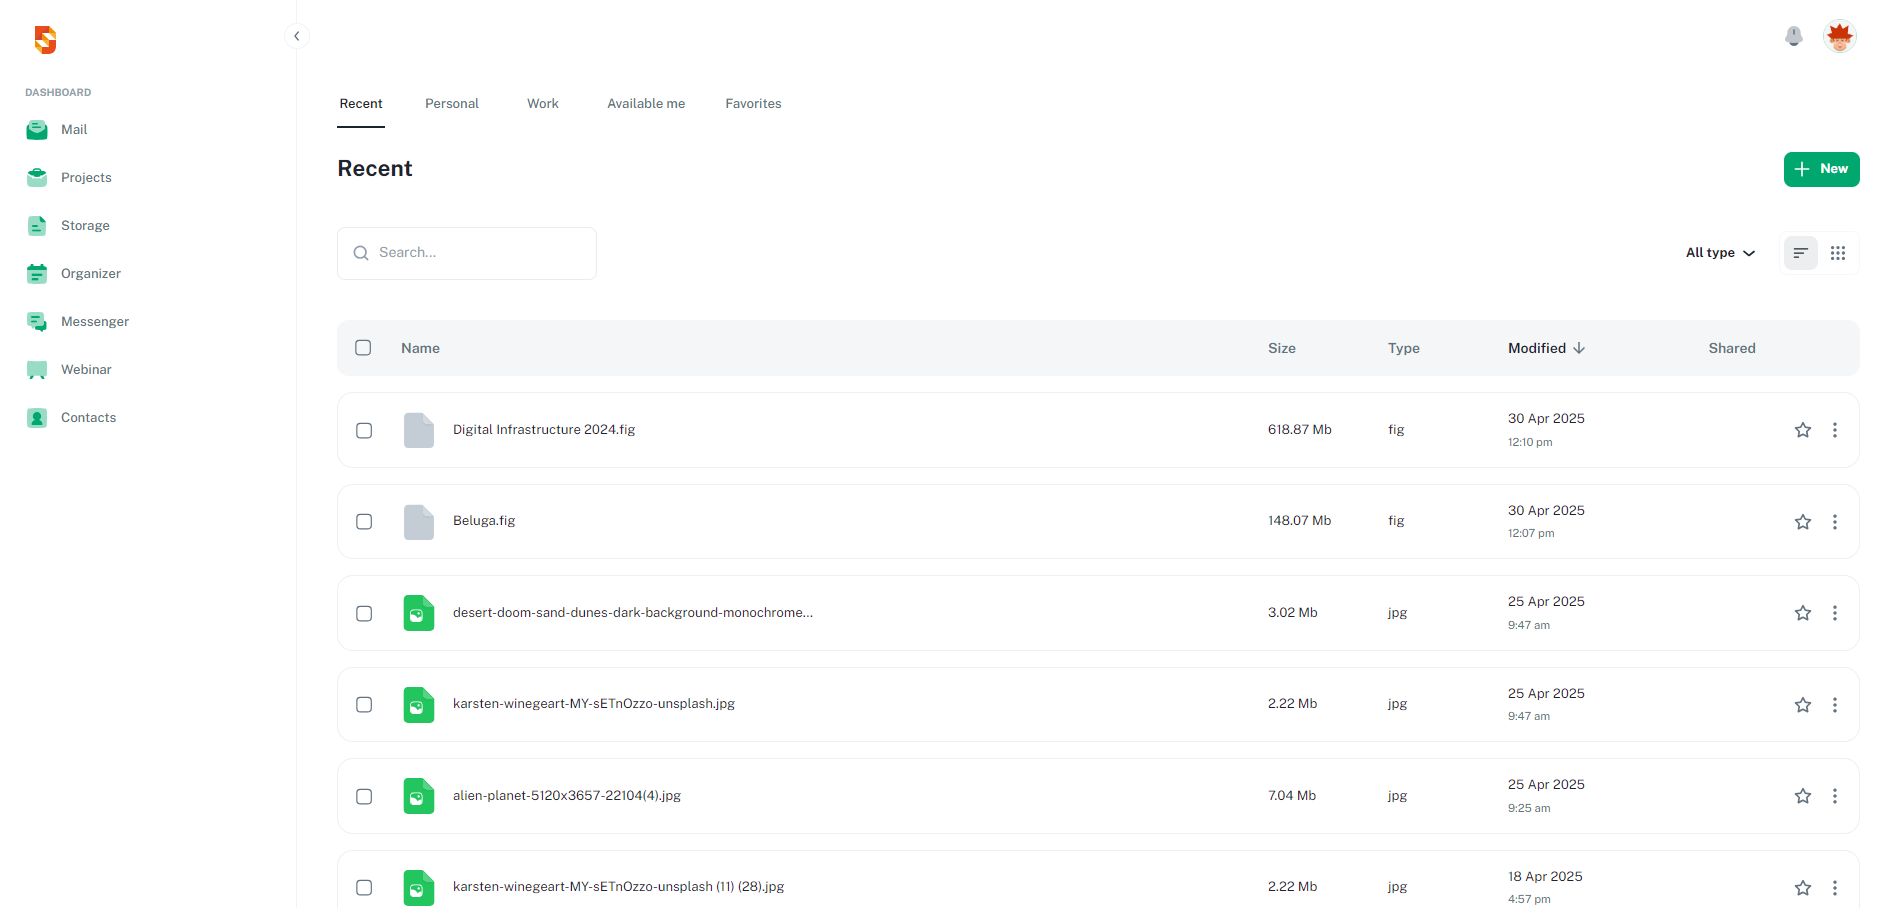
\includegraphics[width=1\linewidth]{images/файлы}
	\caption{Макет интерфейса сервиса <<Файлы>>}
	\label{templ:image9}
\end{figure}

Макет интерфейса создания файла в сервисе <<Файлы>> представлена на рисунке \ref{templ:image9b} и состоит из:
\begin{itemize}
  \item всплывающего окна (1);
  \item поля для ввода названия файла (2);
  \item кнопок действий (3).
\end{itemize}
\begin{figure}[H]
	\centering
	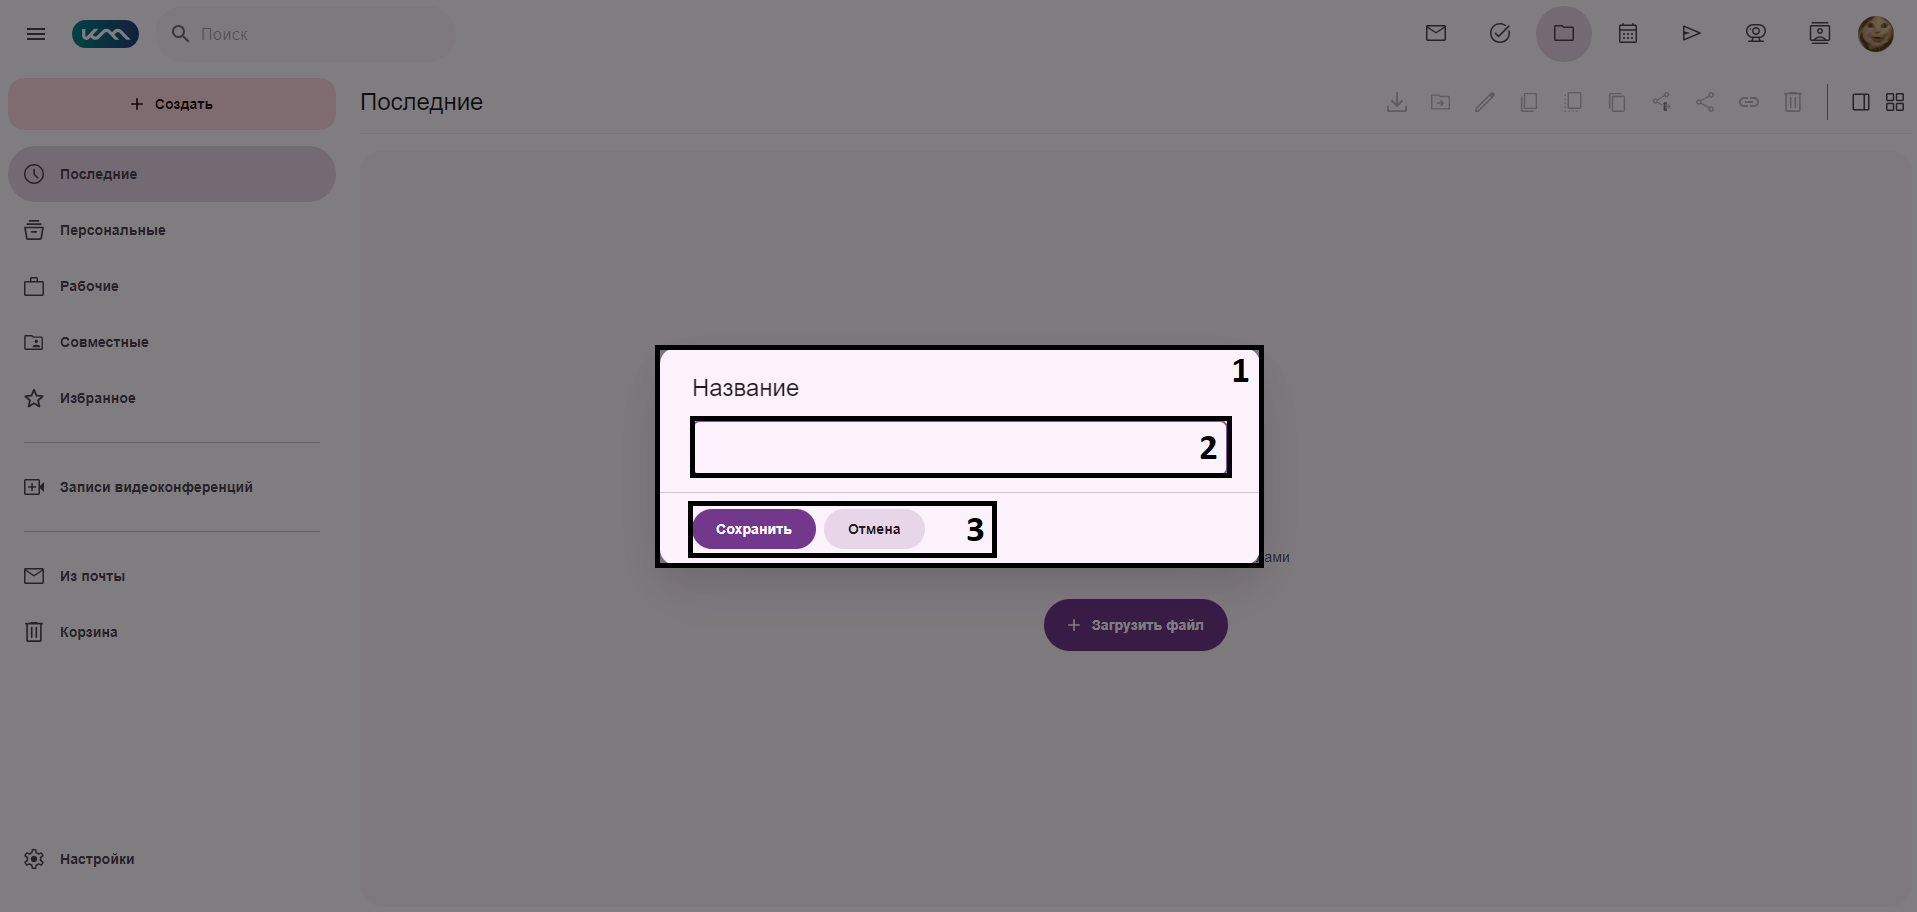
\includegraphics[width=1\linewidth]{images/файлы2}
	\caption{Макет интерфейса создания файла}
	\label{templ:image9b}
\end{figure}

Макет интерфейса загрузки файла в сервисе <<Файлы>> представлена на рисунке \ref{templ:image9c} и состоит из:
\begin{itemize}
  \item всплывающего окна (1);
  \item поля для выгрузки файла (2);
  \item кнопок действий (3).
\end{itemize}
\begin{figure}[H]
	\centering
	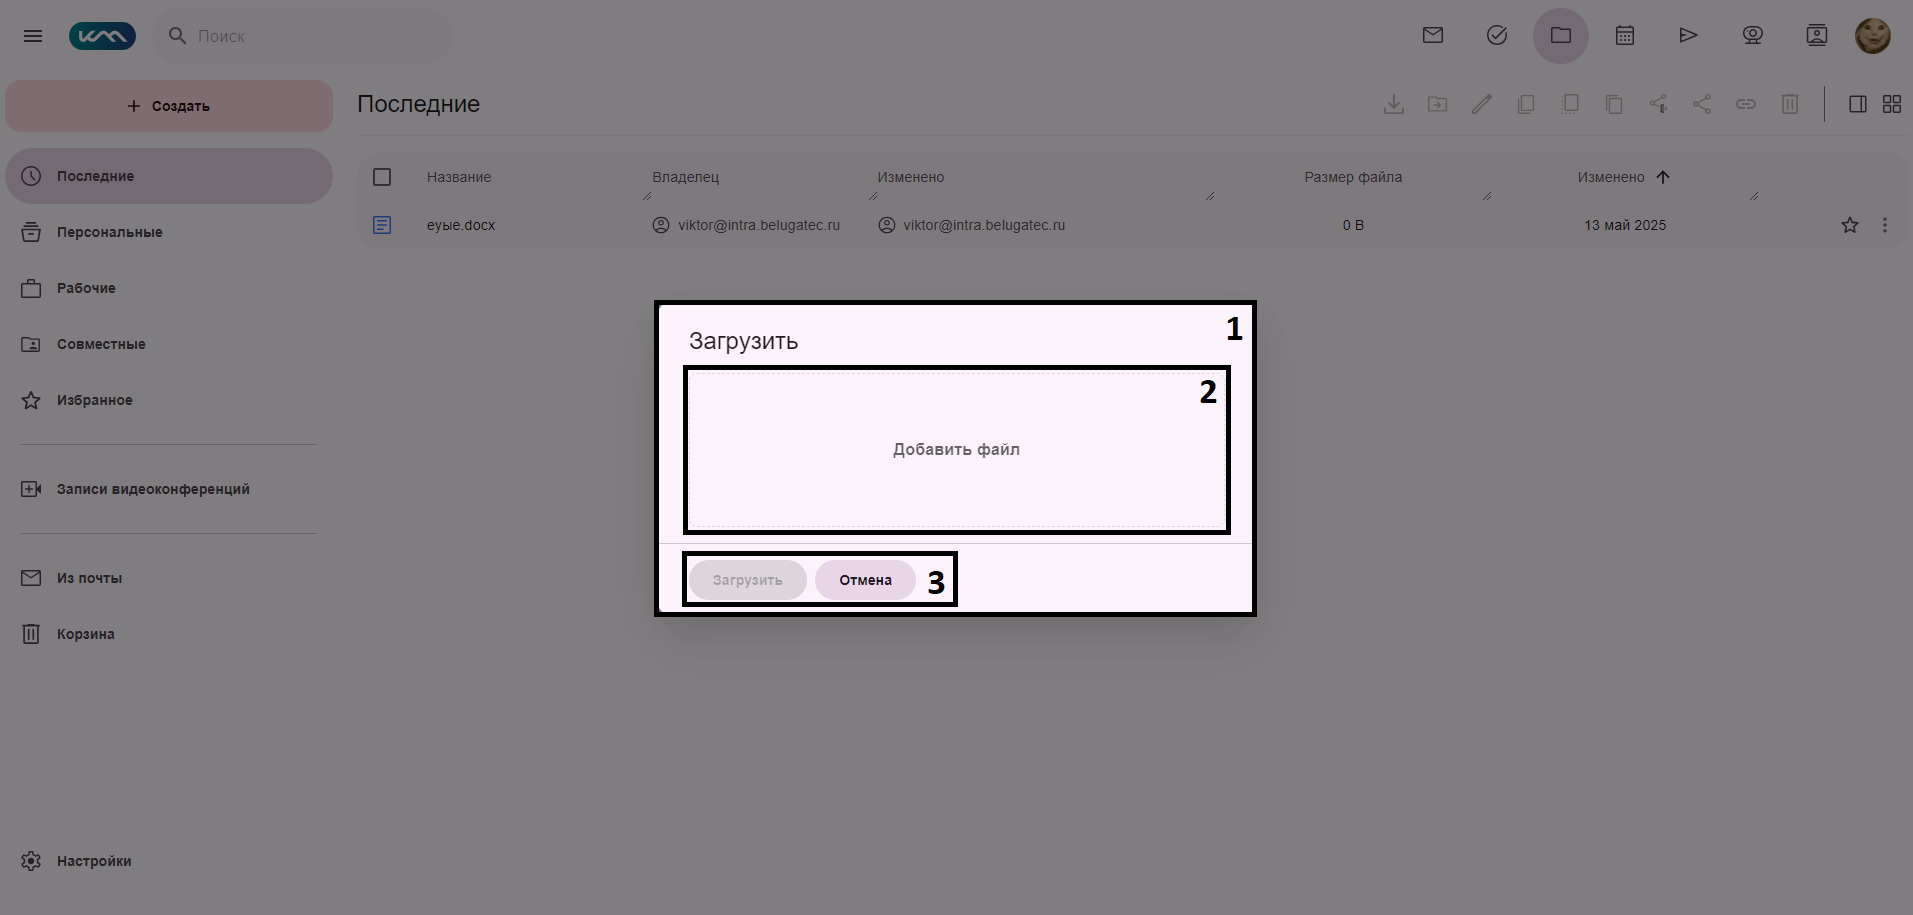
\includegraphics[width=1\linewidth]{images/файлы3}
	\caption{Макет интерфейса загрузки файла}
	\label{templ:image9c}
\end{figure}

Макет интерфейса создания папки в сервисе <<Файлы>> представлена на рисунке \ref{templ:image9d} и состоит из:
\begin{itemize}
  \item всплывающего окна (1);
  \item поля названия папки (2);
  \item кнопок действий (3).
\end{itemize}
\begin{figure}[H]
	\centering
	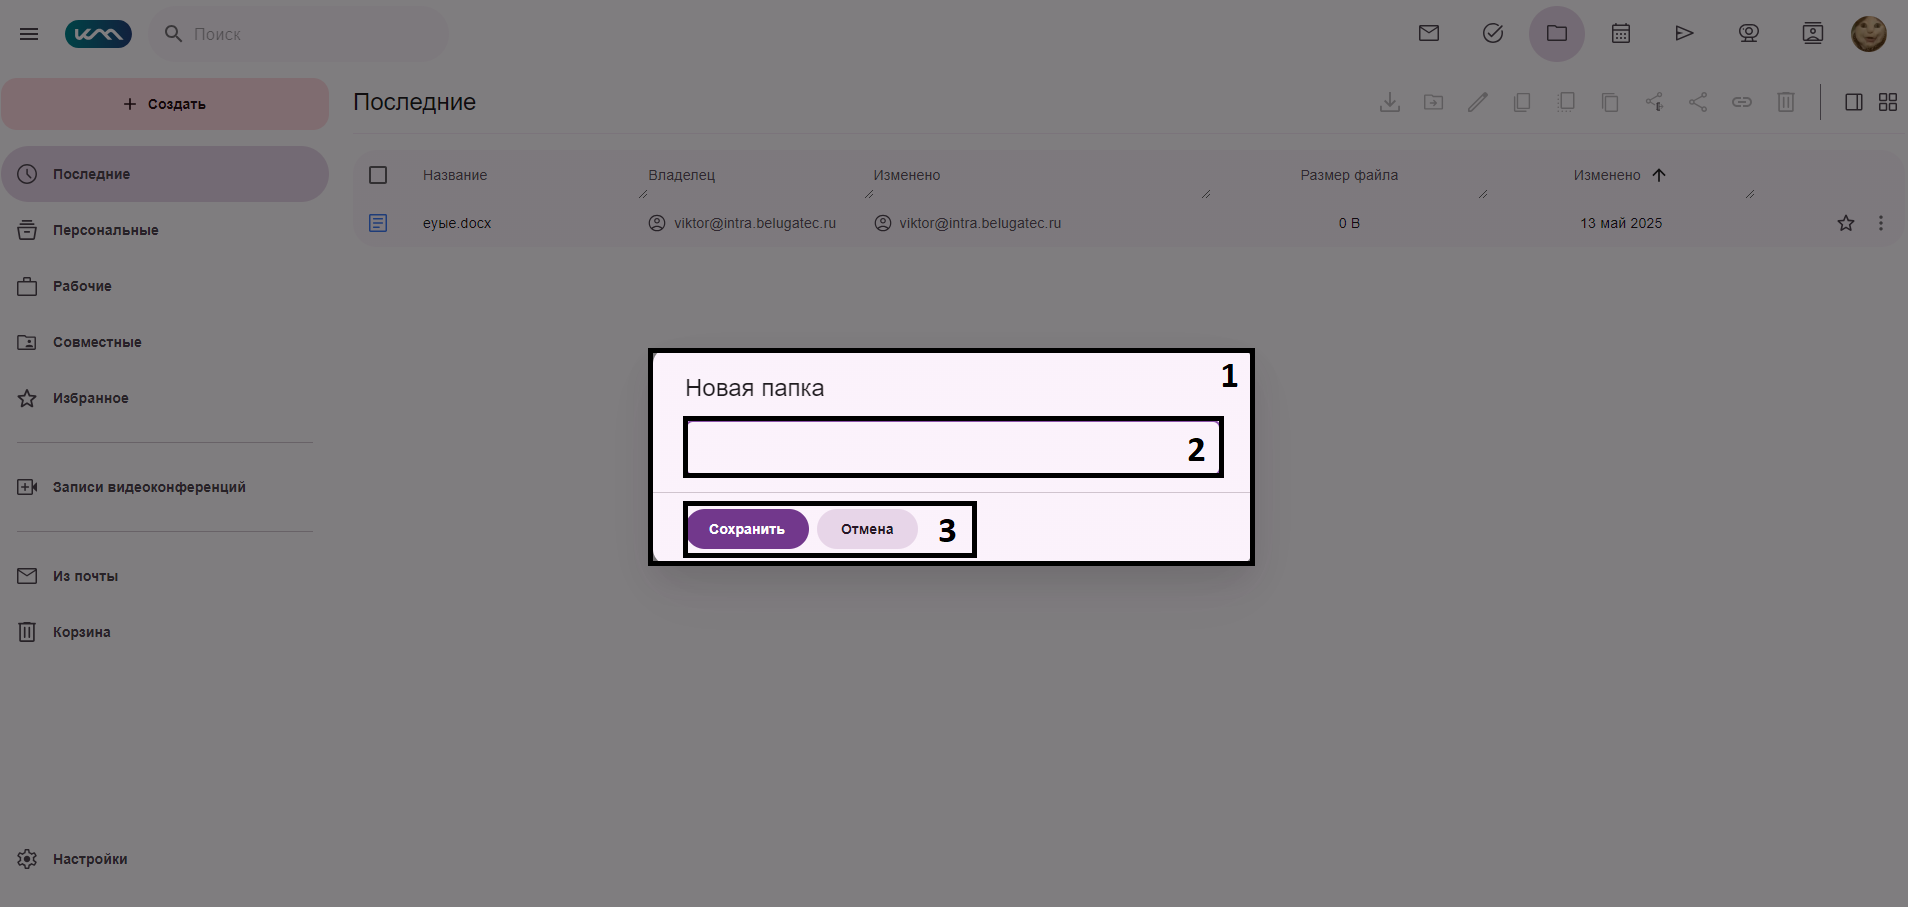
\includegraphics[width=1\linewidth]{images/файлы4}
	\caption{Макет интерфейса создания папки}
	\label{templ:image9d}
\end{figure}

\clearpage
\subsection{Моделирование вариантов использования}

Для разрабатываемой системы была создана модель, которая демонстрирует способы взаимодействия пользователей с программой с помощью унифицированного языка моделирования UML.

На диаграмме вариантов использования система представлена через набор сценариев (прецедентов), с которыми взаимодействуют актёры — пользователи или внешние компьютерные системы. Каждый вариант использования отображается в виде овала с подписью, обозначающей соответствующий сценарий. Эти сценарии описывают, как пользователь может достичь своих целей, взаимодействуя с функциональностью программы. Взаимосвязь между актёрами и вариантами использования показывается через ассоциации.

Применение UML-диаграмм для визуализации работы системы помогает выявить основные взаимодействия и зависимости между компонентами, что облегчает понимание требований, упрощает проектирование и способствует более качественной разработке и тестированию программного обеспечения.

Пользователь с ролью сотрудника имеет доступ ко всем функциональным модулям веб-платформы:
\begin{itemize}
  \item работа с сервисом <<Почта>>;
  \item работа с сервисом <<Разговоры>>;
  \item работа с сервисом <<Проекты>>;
  \item работа с сервисом <<Календарь>>;
  \item работа с сервисом <<Видеоконференцсвязь>>;
  \item работа с сервисом <<Файлы>>;
  \item работа с сервисом <<Контакты>>;
  \item работа с сервисом <<Настройки>>;
  \item работа с сервисом <<Панель управления>>.
\end{itemize}
Эти действия отображены на диаграмме прецедентов, представленной на рисунке~\ref{templ:actor1}.
\begin{figure}[H]
	\centering
	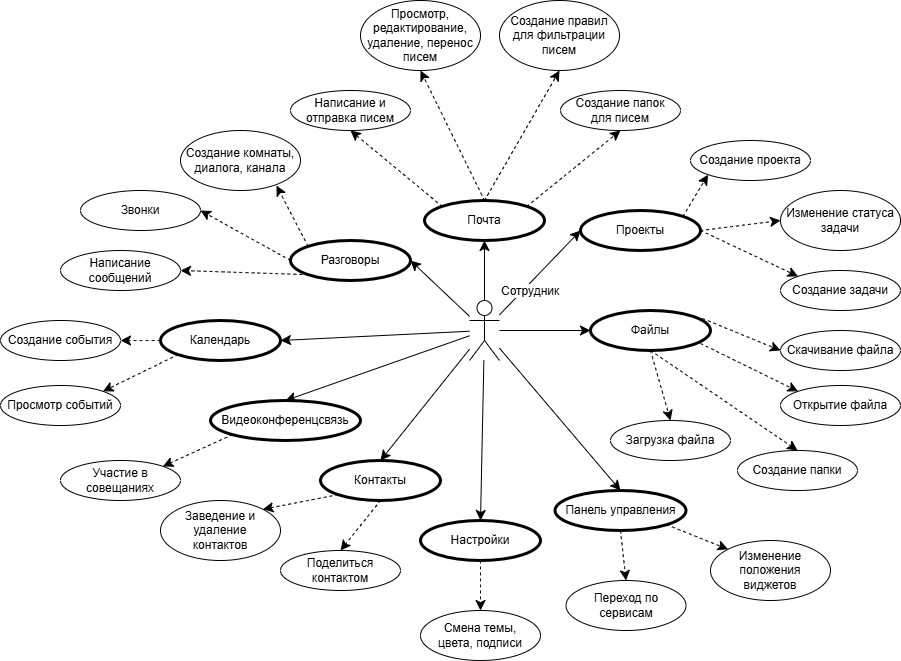
\includegraphics[width=1\linewidth]{images/umldi}
	\caption{Диаграмма прецедентов для сотрудника}
	\label{templ:actor1}
\end{figure}

\subsection{Требования к оформлению документации}

Документация проекта и программного продукта должна оформляться в соответствии с ГОСТ 19.102–77 и ГОСТ 34.601–90. Используемая терминология должна соответствовать принятой в сфере ИТ и быть однозначно понятной.
